\chapter {Formation of Planetary Embryos in the Inner Solar System}\label{ch:plSS}

\noindent \textit{The content of this chapter was originally published in collaboration with Thomas R. Quinn in the October 2019 edition of The Monthly Notices of the Royal Astronomical Society (\cite{wallace19}, MNRAS, Vol. 489, 2; 2019, DOI: 10.1093/mnras/stz2284/), and is reproduced below with the permission of the Royal Astronomical Society.}

\section{Introduction} \label{sec:intro}

The standard scenario of terrestrial planet formation involves the pairwise accretion of small rocky bodies, called planetesimals, 
that condense from dust out of the protostellar disc \cite{safronov69}. \textbf{As discussed in chapter \ref{ch:intro}, the details of growth from cm to km sizes remains uncertain due to fragmentation, bouncing and radial drift barriers \cite{windmark12, weidenschilling77}. However, instabilities that produce large local concentrations of dust and pebbles may provide a way to circumvent these problems \cite{urpin98, youdin05, squire18, squire20}. Assuming larger solids do eventually form, gravity begins tho dominate the physics for objects around a hundred km in diameter.}

\textbf{At this point, gravitational focusing \cite{safronov69} drives runaway growth \cite{duncan89, kokubo96, barnes09} and a handful of relatively large bodies develop. At this point, the largest bodies known as oligarchs, scatter the remaining planetesimals and act to slow the runaway effect. Eventually, the oligarchs accrete most of the available material in the vicinity of their orbit, and space themselves apart by approximately 5-10 Hill radii \cite{kokubo98, kokubo02}. On much longer time scales, the large bodies perturb each other onto crossing orbits, forming Mars to Earth sized bodies via occasional collisions. This phase of late stage accretion is highly chaotic and takes much longer to play out than the previous stages \cite{chambers98, raymond06}.}

%The standard scenario of terrestrial planet formation involves the pairwise accretion of small rocky bodies, called planetesimals, 
%that condense from dust out of the protostellar disc \cite{safronov69}. This accretion process can be broken into a series of 
%distinct stages. First, dust particles settle toward the midplane of the disc and clump together via gravitational instability 
%\cite{goldreich73, youdin02}, streaming instabilities \cite{johansen07, johansen15}, turbulent concentration 
%\cite{chambers10, cuzzi08, cuzzi10, hopkins16} or direct sticking \cite{okuzumi12, windmark12, garaud13, katoka13}. These 
%formation models predict a wide variation in the initial size of planetesimals, ranging from hundreds of meters up to a few 
%hundred kilometers in diameter.

%After this condensation process ends, growth continues via pairwise collisions between planetesimals. Above about 1 km in size, 
%gravitational focusing becomes effective and the collision rate strongly increases. This marks the beginning of the intermediate 
%stage of accretion. During this phase, runaway growth \cite{duncan89, kokubo96, barnes09} quickly increases the size of the 
%largest bodies. Eventually, the largest bodies grow massive enough to heat the small planetesimals, which then inhibits the 
%runaway growth effect. This marks the transition into the phase of oligarchic growth in which the handful of large bodies all tend 
%to grow at the same rate. This produces a bimodal size distribution of planetesimals, with many small bodies and a handful of 
%very large bodies. During this phase, a combination of scattering events between the oligarchs and dynamical friction from the 
%small planetesimals places the oligarchs on nearly circular orbits that are spaced apart by approximately 5-10 Hill radii 
%\cite{kokubo98}. Eventually, the oligarchs accrete most of the available material in the vicinity of their orbit, which eventually 
%throttles their growth rate. On much longer time scales, the large bodies perturb each other onto crossing orbits, forming Mars to 
%Earth sized bodies via occasional collisions. This phase of late stage accretion is highly chaotic and takes much longer to play 
%out than the previous stages \cite{chambers98, raymond06}.

Generally, planetesimal accretion models fail to produce a configuration of planets that resembles that of the Solar System. 
Planets produced in the vicinity of Mars are systematically too massive \cite{wetherill92, raymond09, morishima10, izidoro15} 
and the terrestrial planets that form are too eccentric compared to their Solar System counterparts 
\cite{chambers98, agnor99, chambers01}. In addition, the present day water content of Earth, along with the large D/H ratio of 
Venus \cite{donahue82} does not match with models of solids that condensed out of the Solar nebula at 1 AU.

These issues all have proposed solutions, which generally involve altering the initial conditions for late-stage
accretion simulations. The condition of the Solar System at the beginning of the late stage accretion phase is poorly constrained. 
This is mostly due to the fact that planetesimal formation, and therefore the intermediate accretion phase which produces the 
planetary embryos, is not well understood. Although the present day population of small Solar System bodies has continued to 
evolve since the end of the intermediate accretion phase, the current size frequency distribution (SFD) of asteroid belt and 
Kuiper belt objects contains some clues about the accretion history. \cite{morbidelli09} argued that the SFD of asteroid belt 
objects larger than 100 km in diameter has been largely unchanged, aside from a size independent depletion factor. 
\cite{duncan89} did a long term stability analysis of small Solar System objects and found that small bodies left over from 
accretion should still be largely unperturbed. For these reasons, it should be possible to connect observables in the Solar System to planetesimal formation theories by modeling only the intermediate stages of accretion.

%There are two common ways to model planetesimal growth. A powerful approach is to use statistical methods to track the 
%evolution of large groups of planetesimals. This is known as the particle-in-a-box method \cite{greenberg78, wetherill89}. The 
%evolution of growth is followed by tracking planetesimals in discrete bins of mass and semi-major axis. This removes the need to 
%calculate the motion of every individual body and allows very large collections of planetesimals to be followed. Unfortunately, the 
%dynamics that governs the evolution of these bodies does not always naturally emerge with this approach. 
\textbf{Statistical methods \cite{greenbern78, wetherill89} have proven to be a powerful approach to model planetesimal growth. However, the dynamics governing the evolution of growing planetesimals and protoplanets does not always naturally emerge with this technique.} As an example, 
\cite{weidenschilling11} found that a careful treatment of three body encounters led to a different prediction for the initial size 
distribution of planetesimals near the asteroid belt. Additionally, the particle-in-a-box method is not well suited for studying 
oligarchic growth because the largest mass bins, which dominate the evolution in this stage, contain small numbers of bodies. 
Non-gravitational effects such as gas drag and fragmentation require extra care to implement self-consistently 
\cite{leinhardt08}, although it has been successfully done \cite{wetherill93, chambers01}. To alleviate some of these issues 
while still being able to model large populations, a newer hybrid approach, in which large bodies are treated as single entities 
and planetesimals are treated as statistical ensembles has been developed 
\cite{weidenschilling97, kenyon06, levison12, morishima15}.

The most reliable and straightforward approach is to use N-body methods to follow the evolution and growth of the planetesimals 
\cite{lecar86}. By tracking the individual motions of bodies, the dynamics governing their evolution naturally emerges, no matter 
what the distribution of bodies looks like. However, N-body simulations involving collision detection are extremely 
computationally expensive, which severely limits both the resolution and number of timesteps that can be achieved. This is why 
there are very few studies of runaway and oligarchic with direct N-body simulations in the literature 
\cite{kokubo96, kokubo98, kokubo02, barnes09}. Instead, N-body methods are most commonly used to study late stage 
accretion, where the self-gravity and collisional evolution of the residual planetesimals is largely unimportant 
\cite{chambers98, agnor99,  chambers01, obrien06, morbidelli09}.

To date, we are not aware of any N-body simulations that resolve both the runaway and oligarchic growth phase  with more than 
about $10^4$ particles. At this resolution, stochasticity likely has a significant influence on dynamical friction and resonances 
may not be sufficiently resolved. \cite{raymond06} found that insufficient planetesimal resolution during the oligarchic growth 
phase limits the effectiveness of dynamical friction felt by the oligarchs, producing a population of embryos with unrealistically 
high eccentricities. This idea has also been applied to planet migration through a disc of planetesimals. \cite{cionco02} showed 
that resonances make a significant contribution to the dynamical friction torque exerted by the disc on the planet. This 
phenomenon requires the planetesimals to be finely resolved \cite{brunini07}. Dynamical friction is also facilitated via 
resonances in galactic dynamics \cite{lyndenbell72}. \cite{weinberg07a, weinberg07b} examined the effect of N-body particle 
counts on galaxy dynamics and showed that resonant interactions between the bar and halo were only effective with sufficient 
particle phase space coverage.

For these reasons, we motivate the need for a high resolution N-body simulation of planetesimal growth. We do this to better 
understand the effect that dynamical friction has on the intermediate stages of terrestrial planet growth and to examine what 
predictions a high resolution model makes about the residual population of planetesimals in the Solar System. In particular, 
resonances which are only effective with fine enough resolution, may have an important influence on planetesimal growth. In this 
chapter, we investigate planetesimal evolution during the runaway and oligarchic growth phases with a direct N-body model. We 
begin by simulating an annulus of planetesimals with similar resolution to \cite{kokubo98} to validate our model. We then run the 
same configuration with 100x more particles to better understand the effects of resolution on the intermediate stages of 
terrestrial planet growth.

In section \ref{sec:sim}, we provide a summary of the simulation code, along with a description of the initial conditions used.
In section \ref{sec:plSS_results}, we present the results of the low and high resolution 
simulation of terrestrial planet growth and highlight differences between the two. We find that a bump develops in the mass 
distribution of the high resolution simulation, which does not appear in the low resolution run. This feature manifests itself shortly 
after oligarchic growth commences and we infer that it is produced by extra heating via mean motion resonances between the 
oligarchs and small planetesimals. To further demonstrate this effect, we re-run the high resolution simulation with a narrower 
annulus (depopulating many of the resonances) and show that this reduces the prominence of the bump in the mass distribution. 
In section \ref{sec:dynfric}, we present a set of collisionless simulations of a planetary embryo embedded in an annulus of 
planetesimals. This more clearly demonstrates the differences in dynamical behavior between the low and high resolution 
models. In section \ref{sec:intermed}, we present two more simulations of planetesimal growth at intermediate resolutions and 
demonstrate that the location of the bump is sensitive to the initial planetesimal mass. Finally, section \ref{sec:discussion} 
connects these new results to our present understanding of terrestrial planet growth and we discuss the additional steps 
necessary to use our results to constrain the initial size of planetesimals in the Solar System.

\section{Simulations} \label{sec:sim}

\subsection{Numerical Methods} \label{sec:numerical}

All of the simulations described in this chapter were performed with the highly parallel N-body code {\sc ChaNGa}. A full description 
of the code, along with the details of the solid body collision module are provided in chapter \ref{ch:intro}. For all of the simulations 
presented below, we use a node opening criterion of $\Theta_{BH} = 0.7$. In section \ref{sec:openAngle}, we reduce the value of 
$\Theta_{BH}$ and show that a more accurate and expensive force calculation does not meaningfully affect the timescale for 
viscous stirring.

As in \cite{kokubo96, kokubo98} we accelerate the accretion process by artificially inflating the physical radius of the bodies by 
a factor of $f$. This technique reduces the accretion time-scale by approximately a factor of $f^{2}$, significantly reducing the 
number of timesteps that must be integrated. Additionally, inflating the particle radii allows us to use a smaller annulus with less 
planetesimals. The reason we cannot use an arbitrarily skinny annulus is because the edges tend to expand outward due to the 
unrealistic boundary conditions, decreasing the surface density. The time-scale for this expansion is set by the two body 
relaxation time-scale, which scales with $N$. Reducing the accretion time-scale by increasing $f$ allows us to study 
planetesimal growth with a smaller, less computationally expensive annulus.

We must be careful, however, to choose a value of $f$ that is not too large. The rms eccentricity and inclination of the 
planetesimal disc grows as gravitational encounters transform energy due to Keplerian shear into random motions. By 
accelerating the growth rate, we cause the transitions between growth modes to happen early, when the disc is less dynamically 
excited. This discrepancy is partly compensated for by the fact that our model ignores the effects of gas drag, which would damp 
the eccentricities and inclinations of the planetesimals. We adopt $f=6$ for our calculations, which reduces the amount of 
gravitational scattering by less than 10\% of its true value and does not qualitatively change the modes of planetesimal growth 
\cite{kokubo98}.

\subsection{Initial Conditions} \label{sec:ics}

We begin by using our collision model to perform two sets of calculations:

(i) $10^{6}$ equal mass bodies with $m = 1.2 \times 10^{21}$ g

(ii) 4000 equal mass bodies with $m = 3 \times 10^{23}$ g

\noindent As previously mentioned, simulation (ii) is meant to be compared with the results of \cite{kokubo98}. This allows us to 
both validate our collision model and also have a baseline to compare our simulations to. In both cases, the planetesimals are 
distributed randomly in an annulus centred at 1 AU with a width $\Delta a = 0.085$ AU around a 1 $\mathrm{M_{\odot}}$ star. 
This annulus width was chosen so that the required particle count is minimized without boundary effects influencing planetesimal 
growth. The surface mass density of the ring is set to 10 g cm$^{-2}$, which approximately corresponds to the minimum-mass 
solar nebula model \cite{hayashi81} at 1 AU \footnote{For a discussion of the considerations taken when choosing an initial disk profile, see section 5, chapter 4.}. In case (i), the eccentricities and inclinations are taken from a Rayleigh distribution 
\cite{ida92} with $\langle e^2 \rangle^{1/2} = 2 \langle i^2 \rangle^{1/2} = 4 h/a$, where $h$ is the mutual Hill radius. To match 
the same eccentricity and inclination dispersion with larger planetesimals in case (ii), we use $\langle e^2 \rangle^{1/2} = 2 
\langle i^2 \rangle^{1/2} = 0.635 h/a$. In both simulations, the planetesimals are given an internal density of 2 g cm$^{-3}$. We 
use fixed timesteps with $\Delta T$ = 0.0025 years and evolve the simulations for 20,000 years. Large timesteps diminish the 
effectiveness of gravitational focusing, which inhibits the collision rate. We find that the collision rate is converged below $\Delta 
T$ = 0.0025 years. The integration time was chosen to be comparable to the orbital repulsion and Hill radius growth time-scale 
\cite{kokubo95} so that the effects of oligarchic growth are fully realized by the end of the simulation.

It is worth noting that simulation (i) was a very computationally expensive undertaking. In total, the full 20,000 years of 
integration required approximately 130,000 CPU hours and over 50 days of wall clock time.

\begin{figure}
    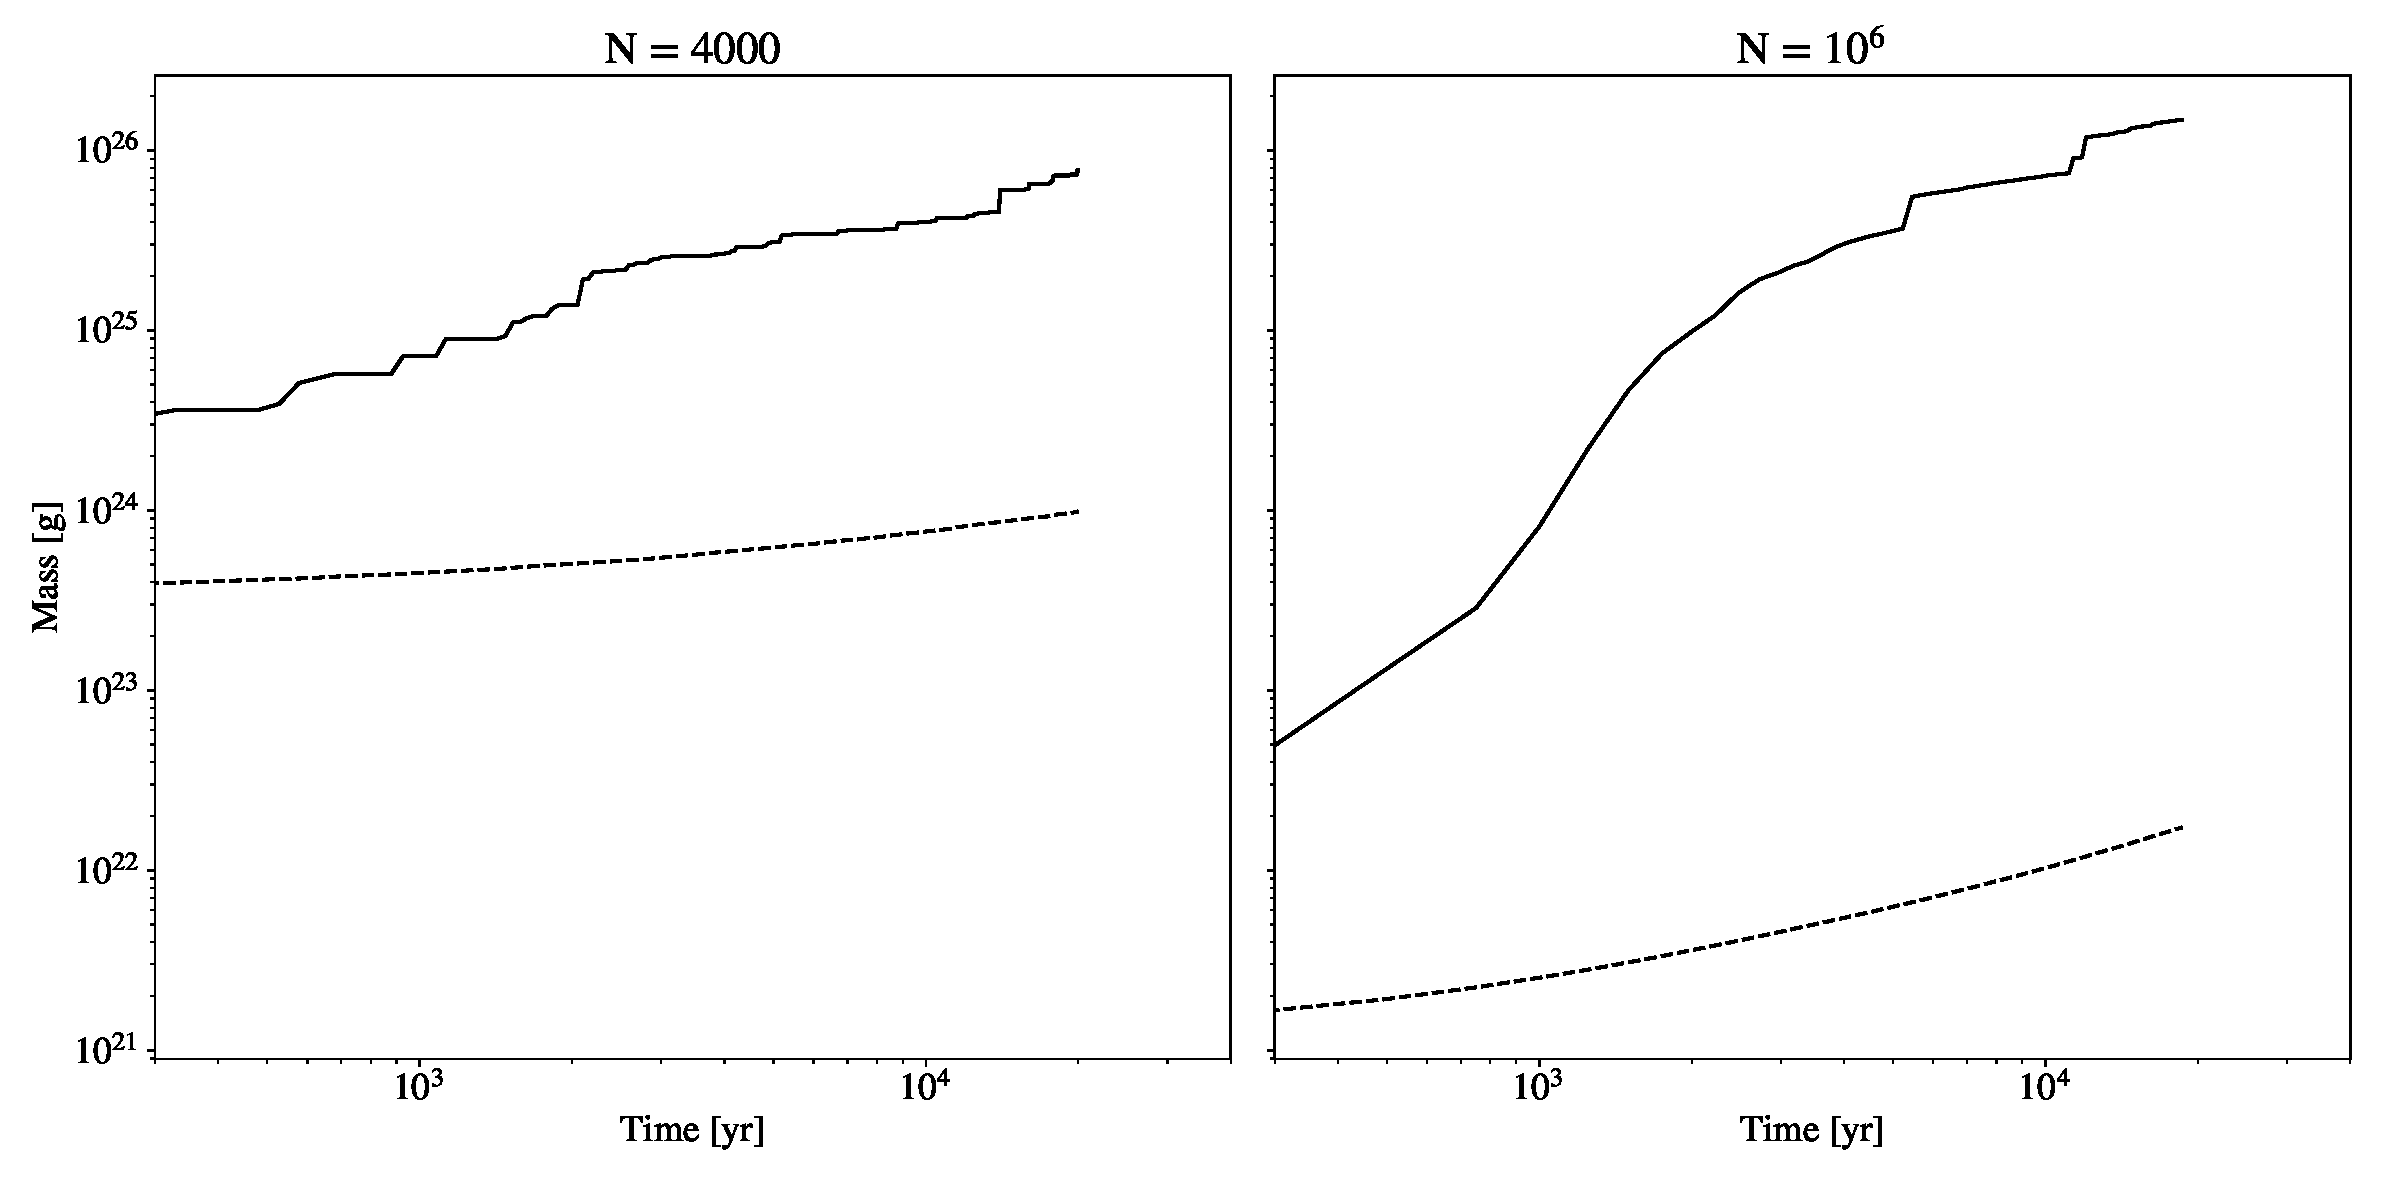
\includegraphics[width=\textwidth]{figures/plSS/mass_evo.eps}
    \caption{Evolution of the maximum (solid curve) and mean (dashed curve) planetesimal mass in the N=4000 and N=$10^6$ particle simulations. At early times, the maximum mass grows more quickly than the mean mass, which is indicative of runaway growth. After a few thousand years, the separation between the curves becomes a constant factor, signalling the start of oligarchic growth.
    \label{fig:mass_evo}}
\end{figure}

\begin{figure}
    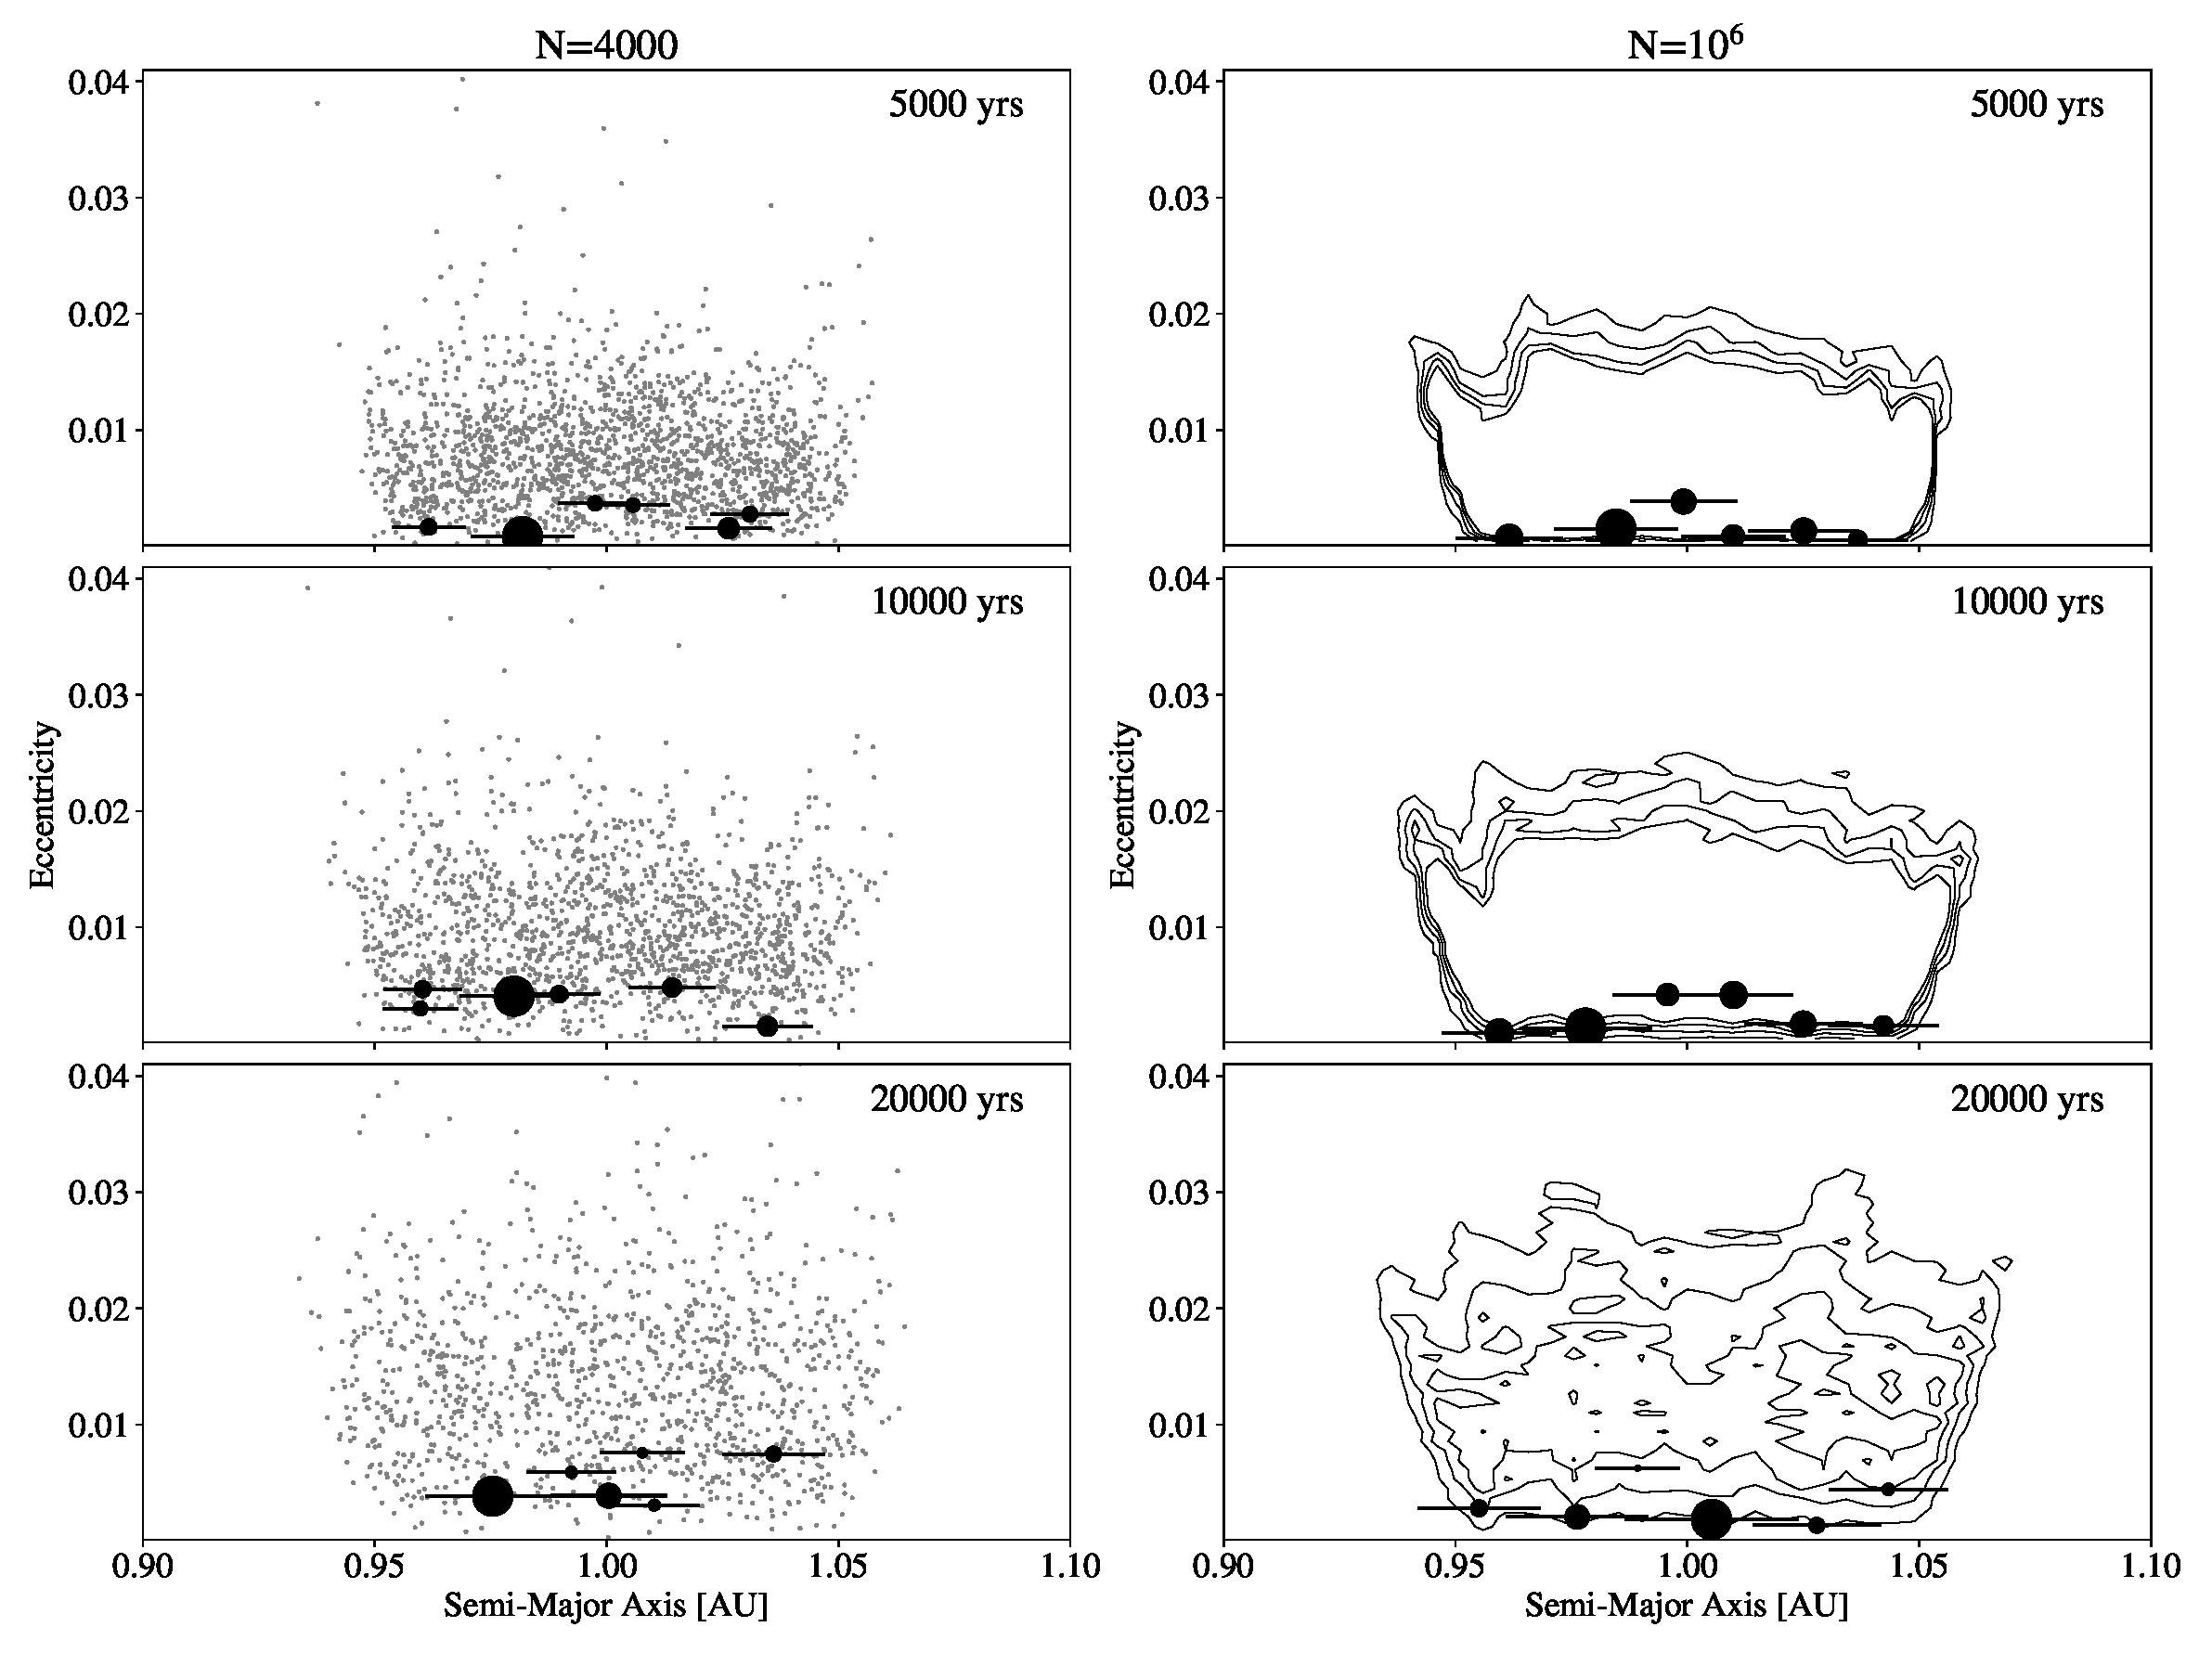
\includegraphics[width=\textwidth]{figures/plSS/ecc_evo.eps}
    \caption{Snapshots from the low and high resolution models in the $a-e$ plane. On the left, the light dots represent individual planetesimals, while the contours on the right hand plots represent curves of constant number density. The contour levels are the same between all panels and correspond to $7.8 \times 10^6$, $1.6 \times 10^7$, $2.3 \times 10^7$, and $3.1 \times 10^7$ planetesimals per AU per unit eccentricity. The black circles denote the configuration of the 6 largest bodies in the simulation, with the area of the circles scaled to the mass of the body. The horizontal error bars are scaled to 5 times the Hill radius of the bodies.
    \label{fig:ae}}
\end{figure}

\begin{figure}
    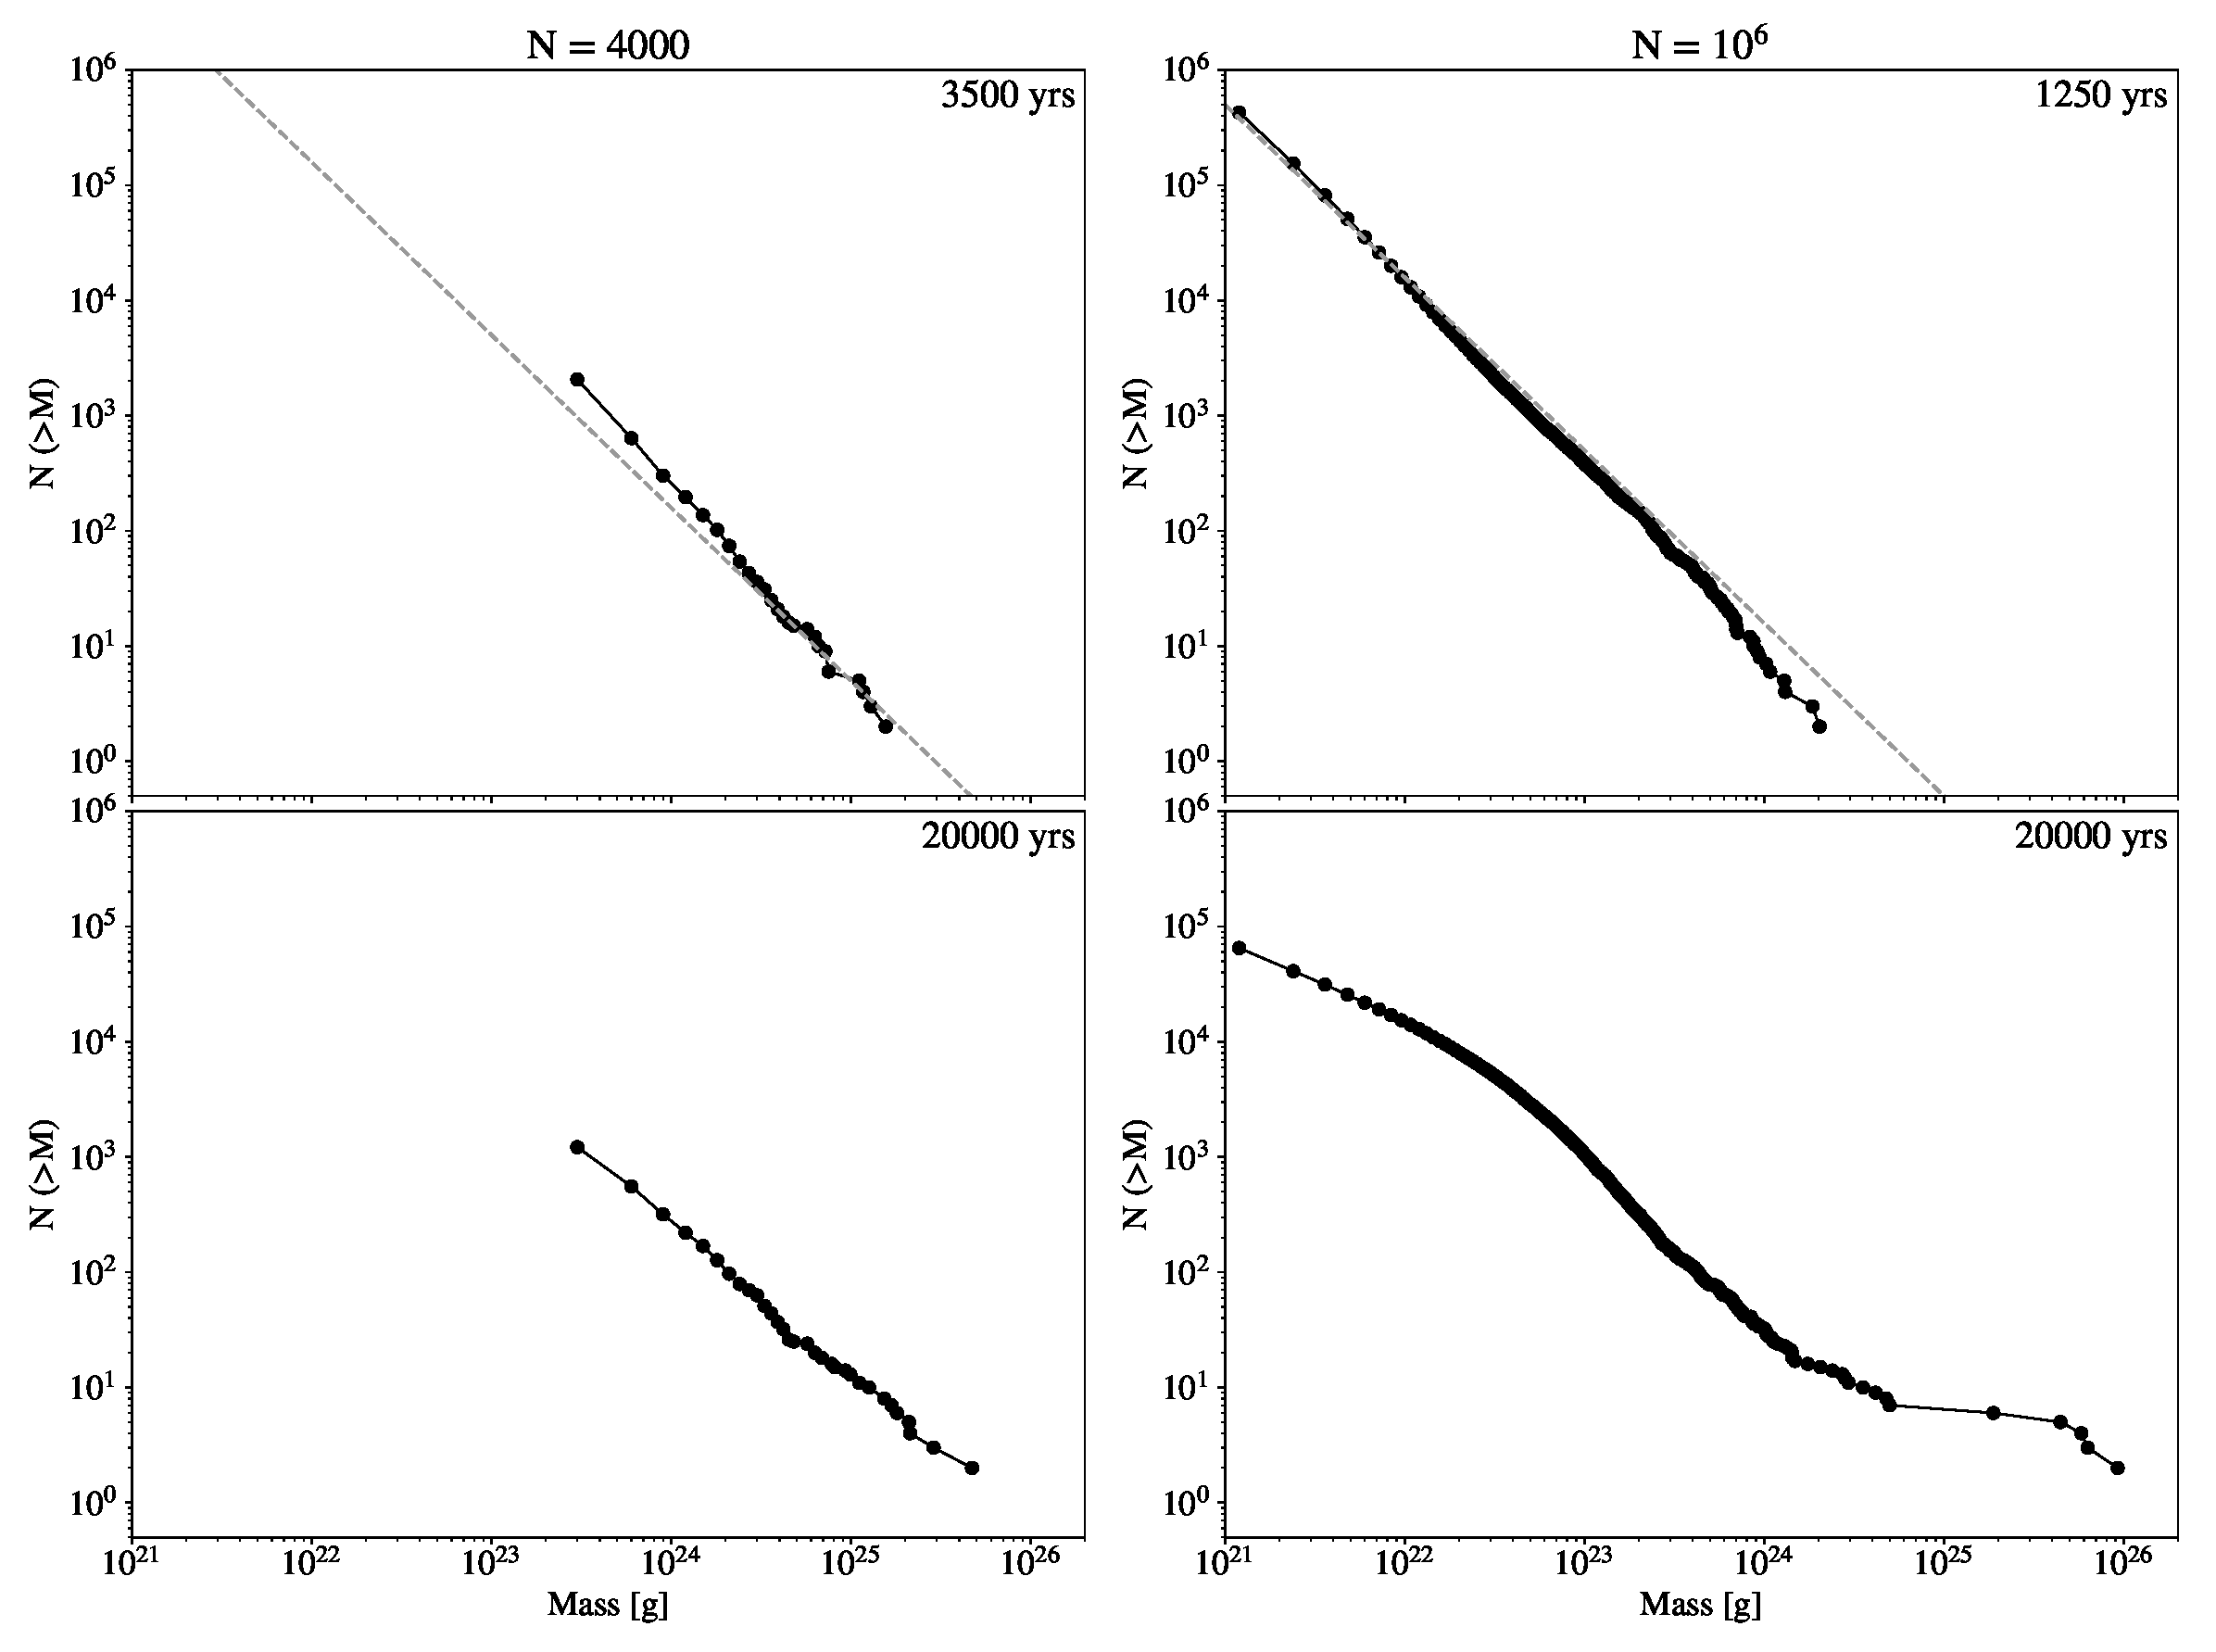
\includegraphics[width=\textwidth]{figures/plSS/mass_spectrum_evo.eps}
    \caption{Cumulative number of bodies in each mass bin for the low and high resolution runs, shown at the end of runaway growth (top row) and the end of the simulation (bottom row). The dashed line indicates a slope of -1.5, which is characteristic of runaway growth \textbf{and can be derived analytically using the coagulation equation \cite{mcleod62, trubnikov71}}. 
    \label{fig:mass_spectrum_evo}}
\end{figure}

\section{Results} \label{sec:plSS_results}

\subsection{Low vs High Resolution}\label{sec:lowvshigh}

We begin by comparing the evolution of growth between the low resolution (N=4000) and high resolution (N=$10^{6}$) models. 
As planetesimals collide and grow, gravitational focusing becomes increasingly effective and the relative growth rate increases 
with mass \cite{greenberg78}. Figure \ref{fig:mass_evo} shows the evolution of the average and maximum planetesimal 
mass in both simulations. Runaway growth at early times is evident from the fact that the maximum mass grows more quickly 
than the mean mass. Eventually, the largest bodies begin to dynamically heat the neighboring planetesimals, which slows the 
growth rate of the largest bodies.

When gravitational focusing and dynamical friction are both effective, the growth rate of a planetesimal of mass $M$ is given by

\begin{equation}\label{eq:growth_rate}
\frac{dM}{dt} \propto \Sigma M^{4/3} e_{m}^{-2},
\end{equation}

\noindent where $\Sigma$ is the surface density of solid material and $e_m$ is the rms eccentricity of the planetesimals 
\cite{kokubo95}. Before the oligarchs form, the eccentricity dispersion is independent of mass and the fractional growth rate 
scales like $dM/dt \propto M^{4/3}$ \cite{wetherill93}. This implies that large bodies grow more quickly than small bodies, hence 
the runaway effect. Once the oligarchs form and dynamical friction becomes effective, energy equipartition causes the velocity 
dispersion to evolve toward $v_m \propto M^{-1/2}$\cite{ida93a}. Using $v_m \propto e_m$ \cite{lissauer93}, the growth rate 
during the oligarchic growth phase scales like  $dM/dt \propto M^{2/3}$. Note that this does not imply that smaller bodies grow 
more quickly than large bodies. Rather, the growth rates tend towards the same value. This is reflected in figure 
\ref{fig:mass_evo}, where the slope of the maximum mass curve flattens out to match the slope of the mean mass curve after a 
few thousand years.

Comparing the two panels in Figure \ref{fig:mass_evo}, it is also evident that the rate of growth is more vigorous in the high 
resolution case. This is due to the fact that the collision time-scale, given by 

\begin{equation}\label{eq:coll_timescale}
t_{coll} = \frac{1}{n \sigma v},
\end{equation}

\noindent is shorter in the latter case, where $n$ is the number density of planetesimals, $\sigma$ is the collision cross section 
and $v$ is the typical encounter velocity. The collision cross section depends on both the geometric cross section ($\propto 
N^{-2/3}$) and an extra term due to gravitational focusing ($\propto N^{-7/3}$), where $N$ is the total number of particles in the 
simulation and the total disk mass \textbf{and geometry} is fixed. Because the eccentricity and inclination dispersion (and therefore the scale height of 
the disk) are kept fixed between the low and high resolution simulations, the typical encounter velocity does not vary with $N$. 
Here, we retain only the leading order term for the collision cross section, in which case these quantities scale like $n \propto N$, 
$\sigma \propto N^{-2/3}$ and $v \propto const$ so that

\begin{equation}\label{eq:coll_timescale_N}
t_{coll} \propto N^{-1/3}.
\end{equation}

Figure \ref{fig:plSS_ae} shows the a-e distribution of planetesimals at three snapshots from both simulations. In both cases, the 
eccentricity dispersion grows as energy from Keplerian shear is transformed into random motion, an effect known as viscous 
stirring \cite{ohtsuki02}. The black circles denote the semi-major axis and eccentricity of the 6 largest bodies. The area of the 
circles indicates the mass of the bodies and the horizontal bars are each scaled to 5 times the Hill radius of the bodies. 
Gravitational scattering between the oligarchs, coupled with dynamical friction from the surrounding planetesimals, places the 
oligarchs on low eccentricity orbits that are spaced apart by a 5-10 Hill radii via orbital repulsion \cite{kokubo98}.

Next, we examine the evolution of the mass distribution of planetesimals. This is shown in Figure \ref{fig:mass_spectrum_evo}. At 
early times, both models exhibit a power law distribution $N(<M) \propto m^{-\gamma}$, where $\gamma$ = 1.5 for the small bodies. A mass 
distribution with this slope is characteristic of runaway growth \cite{wetherill93}. The top panels show the mass distribution from 
both simulations at the end of the the runaway growth phase. In all subsequent snapshots, the mass distribution deviates from a 
single power law as the most massive bodies break away from the distribution, signaling the start of oligarchic growth. This 
happens sooner in the high resolution case. The bottom panels show the mass distribution at the end of the simulation at T = 
20,000 years.

Besides the fact that growth is more vigorous at higher resolution, the final mass distribution of planetesimals in the $N = 10^{6}$ 
case develops a feature that does not appear in the low resolution model. In the low resolution case, the low mass end of the 
mass distribution of planetesimals retains a single power law slope. The high resolution model, on the other hand, develops a 
bump in the mass distribution near $10^{22}$ g.

\begin{figure}
    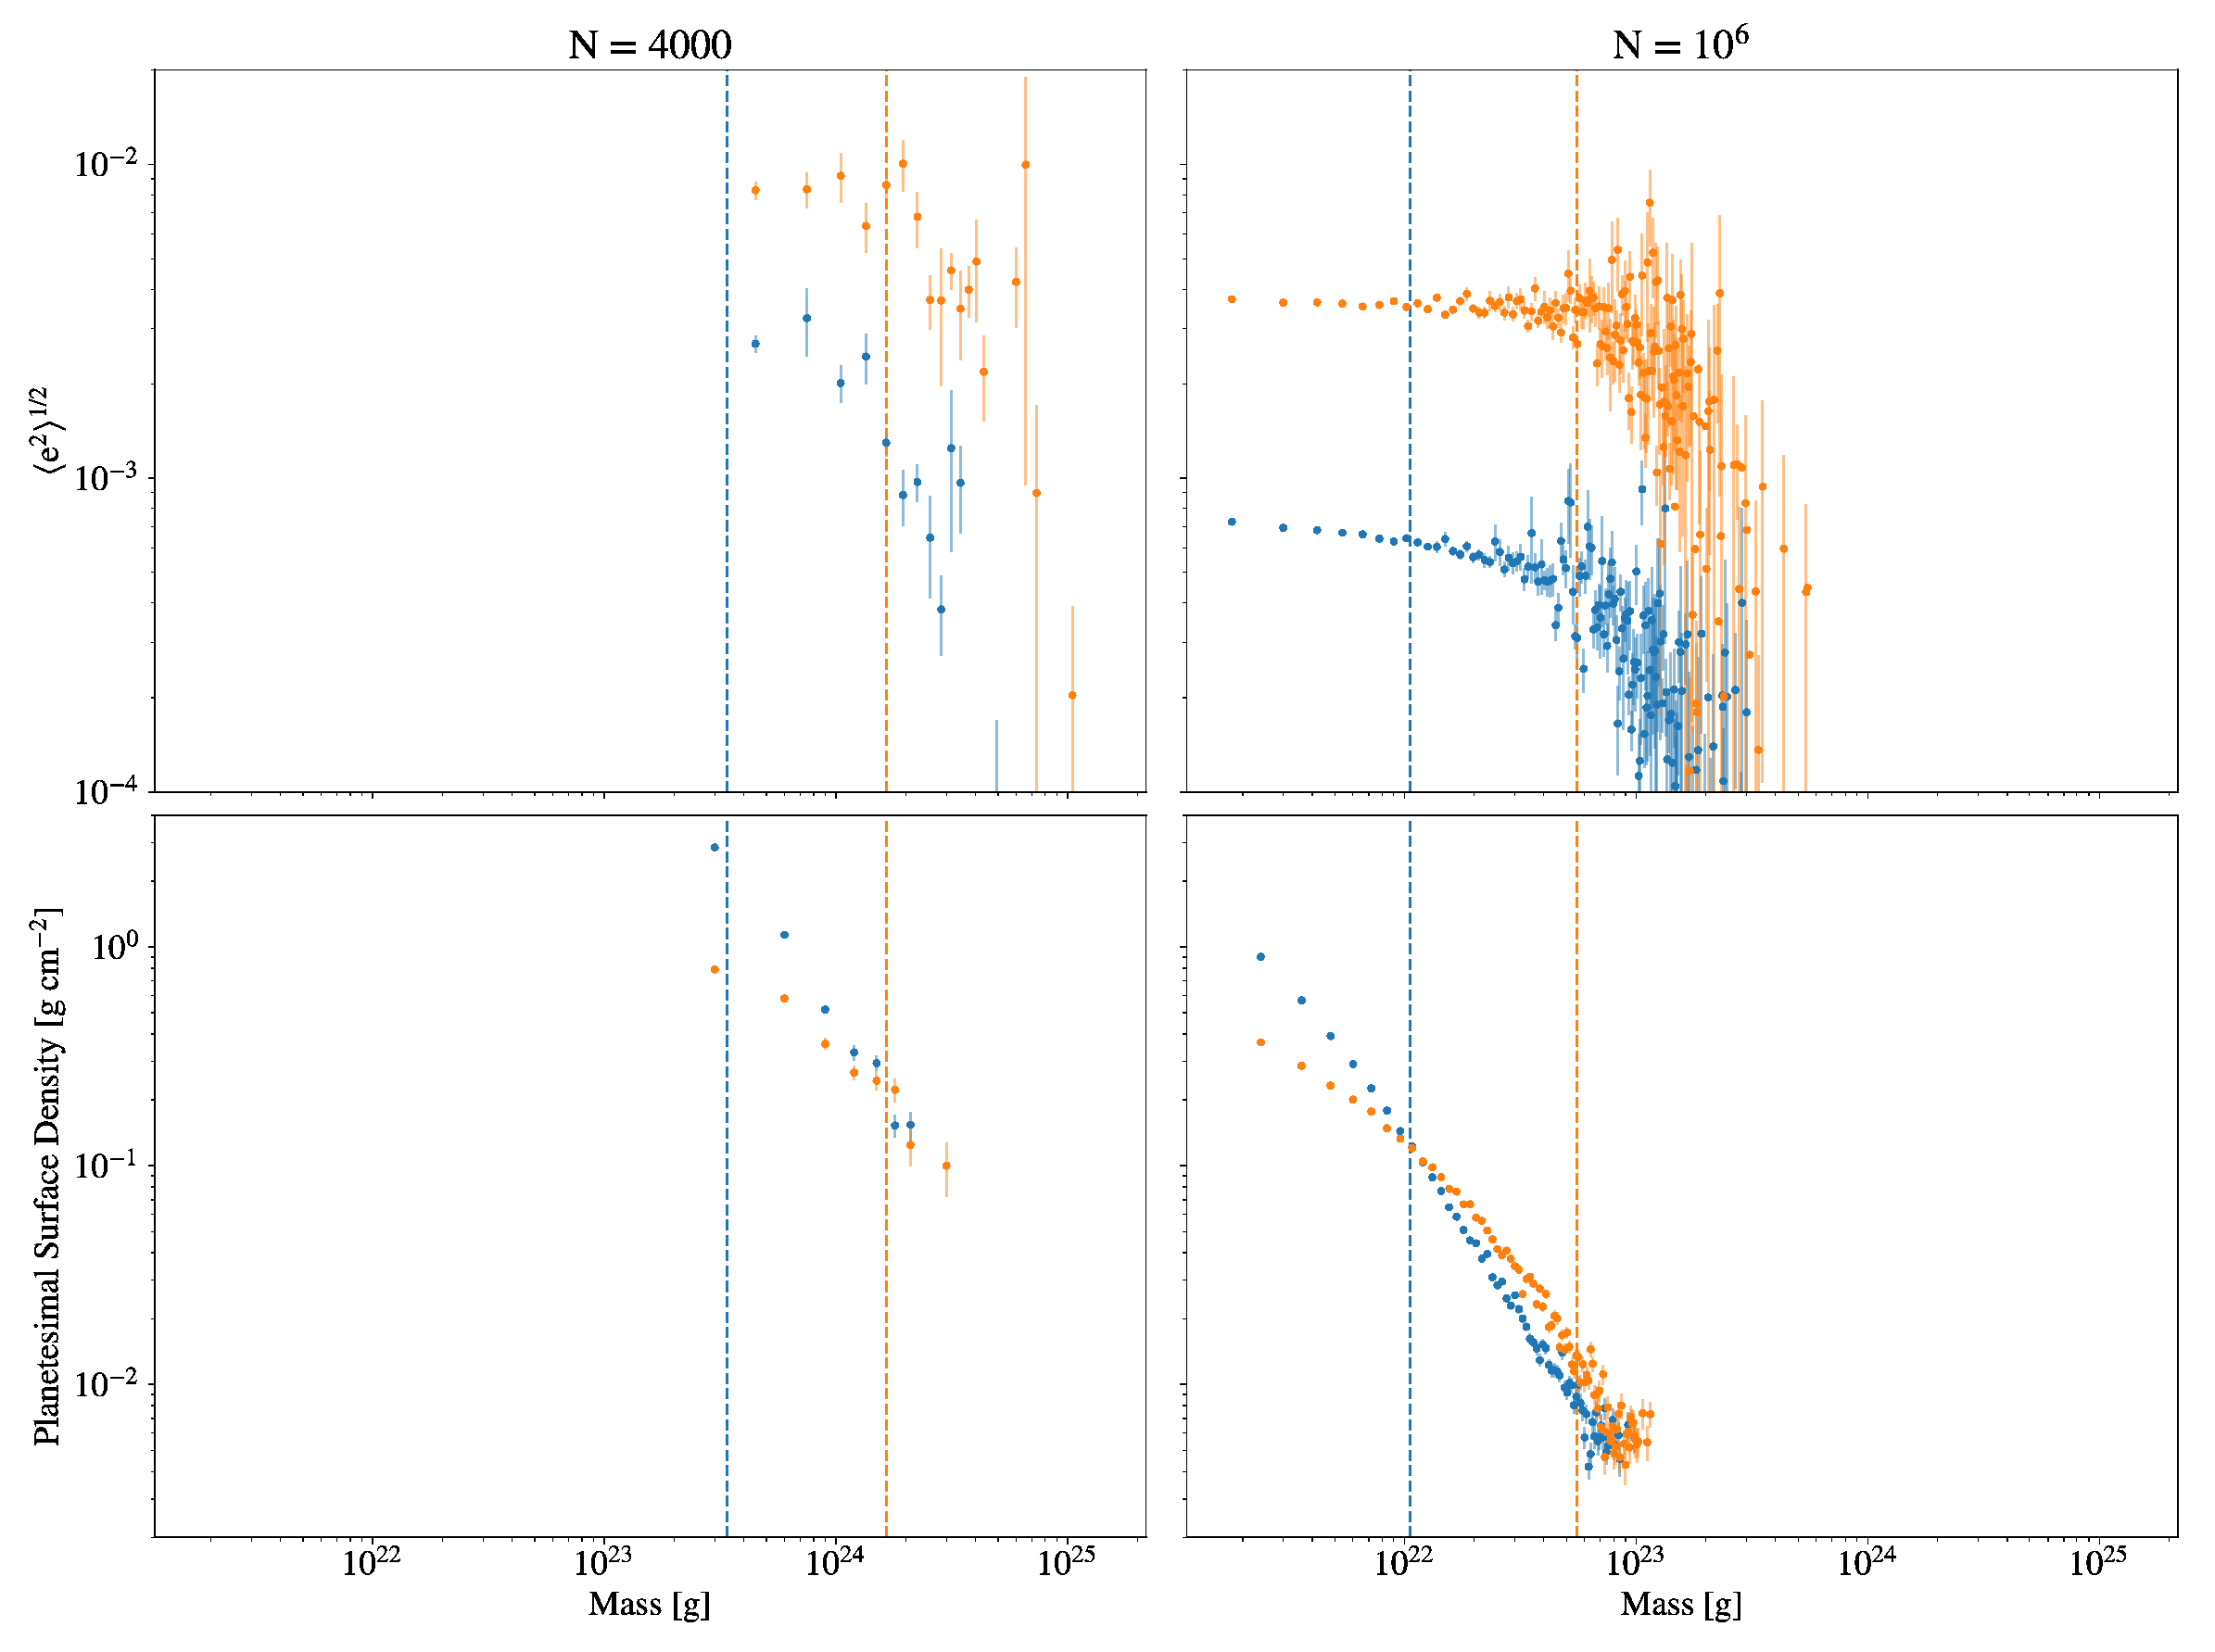
\includegraphics[width=\textwidth]{figures/plSS/ecc_den_evo.eps}
    \caption{The rms eccentricity (top) and planetesimal surface density at each mass (bottom) shown for the $N = 4000$ and 
    $N = 10^6$ simulations. The blue points correspond to the quantities at the end of the runaway growth phase (when the 
    mass distribution deviates from a single power law) and the orange points are from the end of the simulations (T = 20,000 
    years). The vertical dashed lines indicate the value of $M_{stir}$ \textbf{(defined in equation \ref{eq:mstir})} during that snapshot.}
    \label{fig:ecc_den_evo}
\end{figure}

\subsection{Explaining the Bump in the High Resolution Mass Spectrum}\label{sec:bump}

We would next like to determine what produces the feature at $10^{22}$ g in the high resolution simulation and why it is absent 
from the low resolution run. Upon close inspection of the simulation snapshots, both models retain a mass distribution that 
follows a single power law up until the onset of oligarchic growth. The bump in the high resolution mass spectrum becomes 
visible shortly after the oligarchs form. Over the course of the simulation, the bump gradually becomes more prominent. Because 
the bump appears shortly after the first oligarchs do, its presence is likely tied to the formation of the oligarchs.

Other investigations of planetesimal growth have revealed a similar bump in the size frequency distribution (SFD) at intermediate 
masses. \cite{morbidelli09} found that the location of this bump was set by the initial size of the planetesimals. Objects smaller 
than this size were created through disruptive collisions, which resulted in a shallower slope on the SFD to the left of the bump. 
Our collision model does not allow for fragmentation, so we must look for another explanation.

\cite{weidenschilling11} showed that a bump in the SFD was an artefact of the transition between shear and dispersion dominated 
growth. Objects in the shear regime, whose encounter velocities are dominated by the differential rotation of the disc, grow more 
slowly than those in the dispersion regime, whose encounters are set by the random velocity dispersion. Because the velocity 
dispersion varies with planetesimal mass, both of these growth modes can operate simultaneously. Energy equipartition should 
cause the velocity dispersion to decrease with mass, so the transition between shear and dispersion dominated growth should 
happen at some intermediate mass. Finally, the smallest bodies have a velocity dispersion that exceeds their escape velocities, 
which sets a third, slow mode of growth in which gravitational focusing is ineffective. Although our high resolution simulation 
resolves all three modes of growth, we find that the boundaries between these modes smoothly and steadily evolve. Over the 
course of the simulation, the shear-dispersion boundary increases from about $10^{22}$ g to $10^{25}$ g, while the \textbf{boundary at which the encounter velocity exceeds the mutual escape velocity} evolves from about $10^{21}$ to $10^{24}$ g. Any artifacts that these boundaries would leave on the 
planetesimal mass distribution should get washed out, so we also rule these out as explanations for the $10^{22}$ g bump.

Although the boundary between shear and dispersion dominated growth does not seem to be producing the bump, there still 
must be some kind of transition between growth modes occurring near this mass. As shown by equation \ref{eq:growth_rate}, 
the growth rate is controlled by both the surface density of the planetesimals and their eccentricities. In figure 
\ref{fig:ecc_den_evo}, we show the rms eccentricity and surface mass density of the planetesimals as a function of mass at the 
end of the runaway growth phase (blue points) and at the end of the simulation (orange points). In this figure, each point 
corresponds to the relevant quantity calculated for all planetesimals with the exact same mass. Because the simulations start 
with equal mass planetesimals which grow via pairwise collisions, the masses take on discrete, linearly spaced values. We found 
that logarithmically binning the mass values alters the shape of the distributions, especially in the high resolution case where the 
quantities span many orders of magnitude. For this reason, we chose not to bin any of the data. The error bars in figure 
\ref{fig:ecc_den_evo} are obtained via 10,000 iterations of bootstrap resampling. For the high resolution simulation, the error 
bars at low mass are smaller than the size of the points.

The surface density was determined by calculating an azimuthally averaged density profile using the analysis package
{\sc PYNBODY} \cite{pontzen13}. The surface density for each planetesimal mass was taken to be the average surface density 
for those particles in a single radial bin from 0.9575 to 1.0425 AU, which spans the initial boundaries of the annulus.

One might expect that the rms eccentricity spectrum should eventually reach energy equipartition ($e \propto m^{-1/2}$), but this 
has been shown to only occur with a sufficiently steep mass distribution \cite{rafikov03}. In our case, the mass distribution is 
shallow enough that the velocity evolution of the low mass bodies is set only by interactions with large planetesimals. The mass 
below which this occurs, shown by the vertical dashed lines in Figure \ref{fig:ecc_den_evo} is given by
\cite{wetherill93, ormel10}

\begin{equation}\label{eq:mstir}
M_{stir} = \frac{\left< m^2 \right>}{\left< m \right>}.
\end{equation}

Below this mass, planetesimals do not produce a dynamical friction wake and their velocity evolution becomes independent of 
mass \cite{rafikov03}. Because we started with equal mass planetesimals, the mass distribution was steep at early times. A 
power law slope steeper than $\gamma = 2$ should produce a mass-dependent velocity distribution everywhere \cite{rafikov03}. In 
the top right panel of Figure \ref{fig:ecc_den_evo}, the rms eccentricity distribution is not entirely flat below $M_{stir}$, which is 
likely due to the evolving mass spectrum. The analysis of \cite{rafikov03}, however, assumes a static mass spectrum.

At late times, a power law break in the surface density distribution forms near $10^{22}$ g in the high resolution simulation. 
Because the surface density is tied to both the mass distribution and the spatial distribution of planetesimals, it is difficult to learn 
anything else about the dynamics that are altering the growth rate from this information alone. We will examine this further in 
section \ref{sec:dynint}.

Given the power law break in the surface density distribution below $10^{22}$ g, we infer that there must be a dynamical 
mechanism at work that alters the collision rates of the low mass bodies. By the time that the $10^{22}$ g bump begins to 
appear, the planetesimals are sufficiently hot enough to render gravitational focusing ineffective (equation \ref{eq:growth_rate} is 
also no longer applicable). In this case, any additional heating actually increases the collision rate. In the next section, we examine how dynamical friction might be more effective with small planetesimals.

\section{Dynamical Friction and Resolution} \label{sec:dynfric}

Although the Chandrasekhar formula \cite{chandraesekhar43} contains no dependence on particle mass, the 'granularity' of the 
surrounding medium has been shown to influence the action of dynamical friction \cite{brunini07}. This is because the individual 
kicks from gravitational encounters become less frequent and more powerful at coarse resolution, introducing extra stochasticity 
as the system evolves toward energy equipartition. \cite{obrien06} showed that a finely resolved planetesimal distribution during 
the oligarchic growth phase produced planetary embryos with low eccentricities. They did not, however, examine the mass 
spectrum to see if the oligarchs were preferentially heating the smallest planetesimals. In addition, their simulations only 
contained a few thousand particles, while our high resolution run contains in excess of 200,000 bodies at the onset of oligarchic 
growth. Comparing the largest embryos at the end of simulation (i) to their results, we find that the largest embryo in our high 
resolution run has an eccentricity that is a factor of 2 smaller than the embryos produced by \cite{obrien06}.

In addition to altering the cumulative effect of close gravitational encounters, there is evidence that energy and angular 
momentum exchange through resonances is more effective with fine granularity. For example, in collisionless simulations of 
galaxies, \cite{weinberg07a, weinberg07b} showed that a minimum number of particles was required to populate 
resonances and couple the rotation of a bar to the central halo cusp through Lindblad resonances. If the resolution was too 
coarse, gravitational potential fluctuations would scatter particles out of resonances and prevent any strong torque between the 
bar and the halo. Likewise, \cite{cionco02} showed that resonant torque has a measurable effect on the interaction between a 
planet and a planetesimal disc.

\begin{figure}
    \begin{center}
    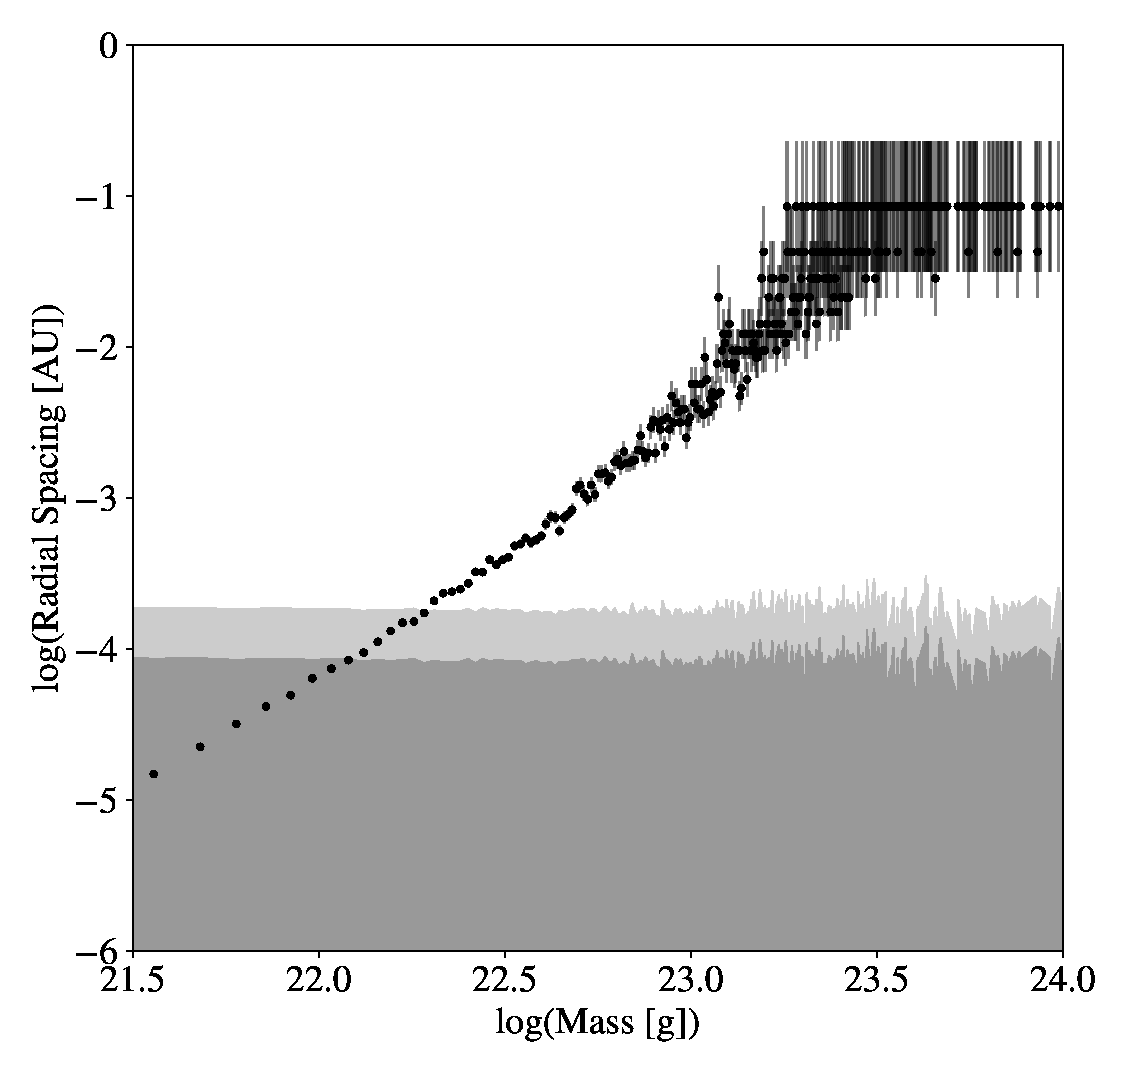
\includegraphics[width=0.5\columnwidth]{figures/plSS/res_width.eps}
    \caption{The average spacing in semi-major axis as a function of mass at the end of the high resolution growth simulation 
    (black points). The gray regions indicate the libration width of planetesimals in each mass bin that are in resonance with the 
    most massive oligarch. The light gray region corresponds to the libration width of the 65:64 (highest non-overlapping) 
    resonance and the dark gray region corresponds to the 15:14 (most distant populated) resonance.}
    \label{fig:res_mass}
    \end{center}
\end{figure}

\subsection{Resolved Resonances}\label{sec:resonances}

During the oligarchic growth phase, a handful of massive bodies lose energy and angular momentum to the surrounding 
medium. The previous runaway growth phase leaves behind a steadily varying spectrum of planetesimal masses, whose number 
decreases with mass. Assuming the planetesimals are randomly distributed throughout the disc, the granularity can be thought 
of as increasing with mass. This implies that the dynamical friction should be more effective from the smallest planetesimals. 
Because the planetesimals appear to be more strongly heated below a certain mass threshold, we hypothesize that the change 
in growth modes has to do with the activation of resonances, rather than a smooth decrease in the stochasticity of scattering 
events.

Because spiral features like those seen in \cite{weinberg07a, weinberg07b} and \cite{cionco02} are unlikely to form in such a 
narrow annulus, we will consider the effects of mean motion resonances (MMRs), which are a subset of the Lindblad resonances 
considered in the aforementioned studies. In order to determine the resolution required to resolve MMRs, we calculate the 
libration width of first order MMRs associated with the oligarchs and compare it to the average radial spacing between 
planetesimals as a function mass. The average radial spacing is given by

\begin{equation}\label{eq:spacing}
\left< \Delta r \right> = \frac{\Delta a}{N(m)},
\end{equation}

\noindent where $\Delta a$ is the width of the annulus and $N(m)$ is the number of planetesimals of each mass.

Because the mass distribution has a negative slope and we expect planetesimals of varying mass to be randomly distributed 
about the disc, the radial spacing between planetesimals should increase with mass. For a fixed resonance width, there should 
be a cutoff in mass, below which planetesimals are more strongly affected by the resonances. The libration width of a first order 
mean motion resonance can be derived analytically using the pendulum approximation \cite{murray00} and is given by

\begin{equation}\label{eq:lib_width}
\frac{\delta a}{a} = \pm \left(\frac{16}{3} \frac{\left| C_{r} \right|}{n} e \right)^{1/2} \left(  1 + \frac{1}{27 j_{2}^2 e^3} \frac{\left| C_{r} \right|}{n} \right)^{1/2} - \frac{2}{9 j_{2} e}  \frac{\left| C_{r} \right|}{n},
\end{equation}

\noindent where $a$ is the semi-major axis at the center of the resonance, $e$ is the eccentricity of the body in resonance and 
$j_2 = -q$ where $p:q$ is the MMR being considered. $\left| C_{r} \right|/n = (m^{\prime}/m_{c}) \alpha f_{d}(\alpha)$, where $
(m^{\prime}/m_{c})$ is the mass ratio of the body associated with the resonance to the central body, $\alpha$ is the semi-major 
axis ratio associated with the resonance and $f_{d}(\alpha)$ is the disturbing function. For an interior first order resonance, the 
disturbing function can be expressed as

\begin{equation}\label{eq:dist}
f_{d}(\alpha) = j b_{1/2}^{j} + \frac{\alpha}{2}\frac{d b_{1/2}^{j}}{d \alpha},
\end{equation}

\noindent \cite{winter97} where $j = 1 - j_{2}$ and $b_{1/2}^{j}$ is a Laplace coefficient which is defined as

\begin{equation}\label{eq:lap}
b_{s}^{j}(\alpha) = \frac{1}{2 \pi} \int_{0}^{2 \pi} \frac{cos \, j \theta \, d \theta}{\left( 1 - 2 \alpha \, cos \theta + \alpha^2 \right)^{s}}.
\end{equation}

\noindent The derivative in the second term of equation \ref{eq:dist} can be written in terms of the Laplace coefficients 
\cite{murray00}

\begin{equation}\label{eq:lap_d}
\frac{d b_{s}^{j}}{d \alpha} = s \left( b_{s+1}^{j-1} - 2 \alpha b_{s+1}^{j} + b_{s+1}^{j+1} \right).
\end{equation}

\textbf{One should exercise caution, however, when using a perturbative approach to understand resonant behavior at small eccentricities. Naively, one might interpret equation \ref{eq:lib_width} to imply that the width of a first order interior MMR grows to infinity as $e \to 0$. Instead, recent non-perturbative numerical analyses have shown that these resonances instead split into pericentric and apocentric branches, which diverge away from the nominal resonance location and have a very narrow radial and azimuthal extent \cite{malhotra23}. The mass ranges relevant for our growing planetesimal disk have yet to be explored in this context (see \cite{malhotra22} for a review). However, the dynamical heating that naturally emerges due to repeated gravitational interactions between protoplanets and planetesimals should act to keep resonant bodies out of this low-eccentricity regime.}

Figure \ref{fig:res_mass} shows the libration width and average radial spacing of the planetesimals as a function of mass at the 
end of the high resolution run. To calculate the libration width as a function of planetesimal mass, the $e$ used in equation 
\ref{eq:lib_width} was taken to be the average eccentricity in each mass bin, while $a$ was set to the semi-major axis of the 
largest oligarch in the simulation. The slight variation in the resonance width as a function of mass is due to the variation in 
eccentricity. The error bars on the radial spacing data are calculated from Poisson statistics.

This calculation was done for the 15:14 and 65:64 mean motion resonances. The 15:14 resonance is the most distant first order 
resonance relative to an oligarch at 1 AU that still lies within the annulus of planetesimals. The 65:64 resonance is the closest 
MMR for which the libration width is smaller than the spacing between resonances. Higher first order resonances should not 
exhibit any resolution dependence because they overlap. For planetesimals less massive than about $10^{22}$ g, the average 
particle spacing drops below the libration width. Bodies below this mass cutoff, which we will refer to as the resonance heating 
mass $M_{res}$, are more likely to populate MMRs. This provides an explanation for how the oligarchs are preferentially heating 
the low mass bodies. Comparing with Figure \ref{fig:ecc_den_evo}, the mass of the power law break in the surface density 
matches very closely with $M_{res}$, which also matches the location of the $10^{22}$ g bump in figure 
\ref{fig:mass_spectrum_evo}. Over the course of the simulation, $M_{res}$ increases by no more than a factor of 2, so the 
growth mode boundary could easily leave an imprint on the mass spectrum, unlike the shear/dispersion dominated growth 
boundary, which evolves from $10^{22}$ to $10^{25}$ g.

In the restricted three-body problem, the orbital parameters of a test particle receiving energy and angular momentum via a 
mean motion resonance will evolve such that

\begin{equation}\label{eq:tiss}
\frac{de}{da} = \frac{a^{3/2} - 1}{2 a^{5/2} e},
\end{equation}

\noindent where $a$ is in units relative to the semi-major axis of the perturbing body. In the above equation, the inclination is 
assumed to be negligibly small \cite{murray00}.

Equation \ref{eq:tiss} can be used to place an upper limit on the change in eccentricity that a planetesimal in resonance will 
experience. Because any $\delta a$ larger than the resonance width will remove the planetesimal from the resonant influence of 
the oligarch, $\delta e$ is also restricted by the resonance width. Taking $a \approx 0.95$ (the location of the 15:14 resonance), 
$e \approx 10^{-3}$ and $\delta a \approx 10^{-4}$ (the libration width of the 15:14 MMR) we predict a first order change in 
eccentricity of $10^{-4}$. This value is small relative to the rms eccentricity of the planetesimals, which explains why the effects 
of the  mean motion resonances are not visible in Figure \ref{fig:plSS_ae} or in the top right panel of Figure \ref{fig:ecc_den_evo}.

\begin{figure}
    \begin{centering}
    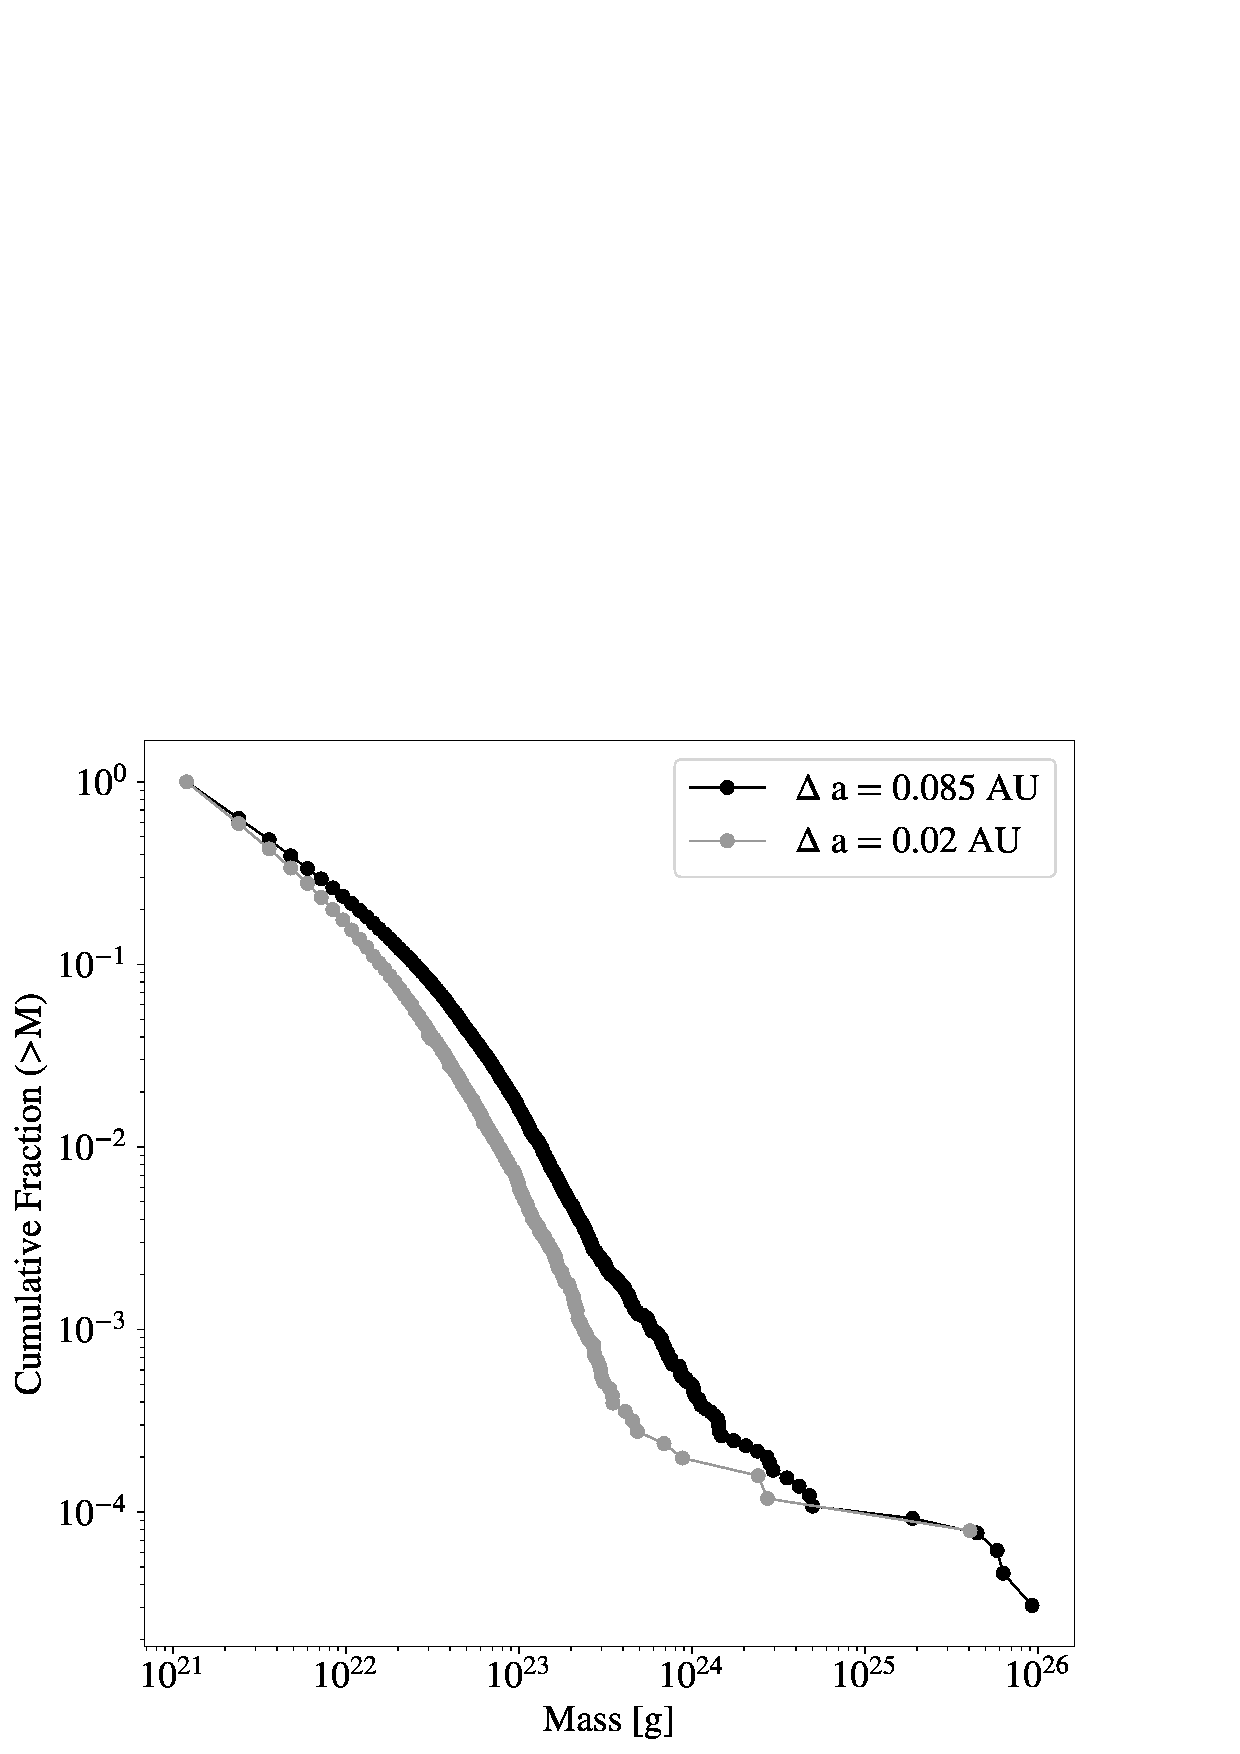
\includegraphics[width=0.5\columnwidth]{figures/plSS/mass_spectrum_comp.png}
    \caption{The cumulative fraction of bodies as a function of mass in the wide (solid dark curve) and narrow (gray curve) high 
    resolution growth simulations. Decreasing the annulus width, which depopulates resonances, produces a less prominent 
    $10^{22}$ g bump. The dashed black line shows the mass spectrum predicted  by a runaway growth scenario using the coagulation equation \cite{mcleod62, trubnikov71}.}
    \end{centering}
    \label{fig:mass_spectrum_comp}
\end{figure}
Because the resonances are not possible to pick out by eye on an $a-e$ plot, we ran a modified version of simulation (i), the 
purpose of which is to show how planetesimal growth proceeds when the mean motion resonances are not present. The initial 
conditions are identical to those described in section \ref{sec:ics}, except that the annulus only extends from 0.98 to 1.02 AU. 
This effectively depopulates all of the first order mean motion resonances below the 26:25 resonance. It was not possible to use 
an annulus skinnier than this without introducing strong boundary effects which influence the growth of the planetesimals. This 
makes it impossible to depopulate all of the resolved resonances. The mass spectrum at the end of the skinny annulus 
simulation (also evolved for 20,000 years), along with the mass spectrum at the end of the high resolution growth simulation, is 
shown in Figure \ref{fig:mass_spectrum_comp}. With a narrower annulus, the change in slope of the mass distribution below 
$10^{22}$ g is noticeably weaker. We attribute this to the fact that the resonant interaction between the planetesimals and 
oligarchs is diminished because many of the MMRs are now empty.

\subsection{Planetesimal and Oligarch Mixing}\label{sec:mix}

Although figures \ref{fig:res_mass} and \ref{fig:mass_spectrum_comp} provide \textbf{circumstantial} evidence that the $10^{22}$ g bump is 
being produced by mean motion resonances, it is not immediately clear how the resonances affect such a large fraction of the 
planetesimals. To have a noticeable effect on the mass distribution, the oligarchs must be affecting bodies below $M_{res}$ 
everywhere in the disc, not just within the small fraction of space covered by the MMRs at a given time.

We infer that both the oligarchs and planetesimals slowly wander through the annulus due to occasional scattering events. This 
continually replenishes the population of planetesimals that are sitting inside of resonances. The orbital repulsion effect 
described by \cite{kokubo98}, which moves the oligarchs around, alters the location of the mean motion resonances. 
In addition, we infer that the planetesimals are occasionally scattered by the oligarchs. These two effects slowly cycle different 
planetesimals through the resonances and allow the oligarchs to eventually heat a large fraction of the small bodies.

\begin{figure}
    \begin{centering}
    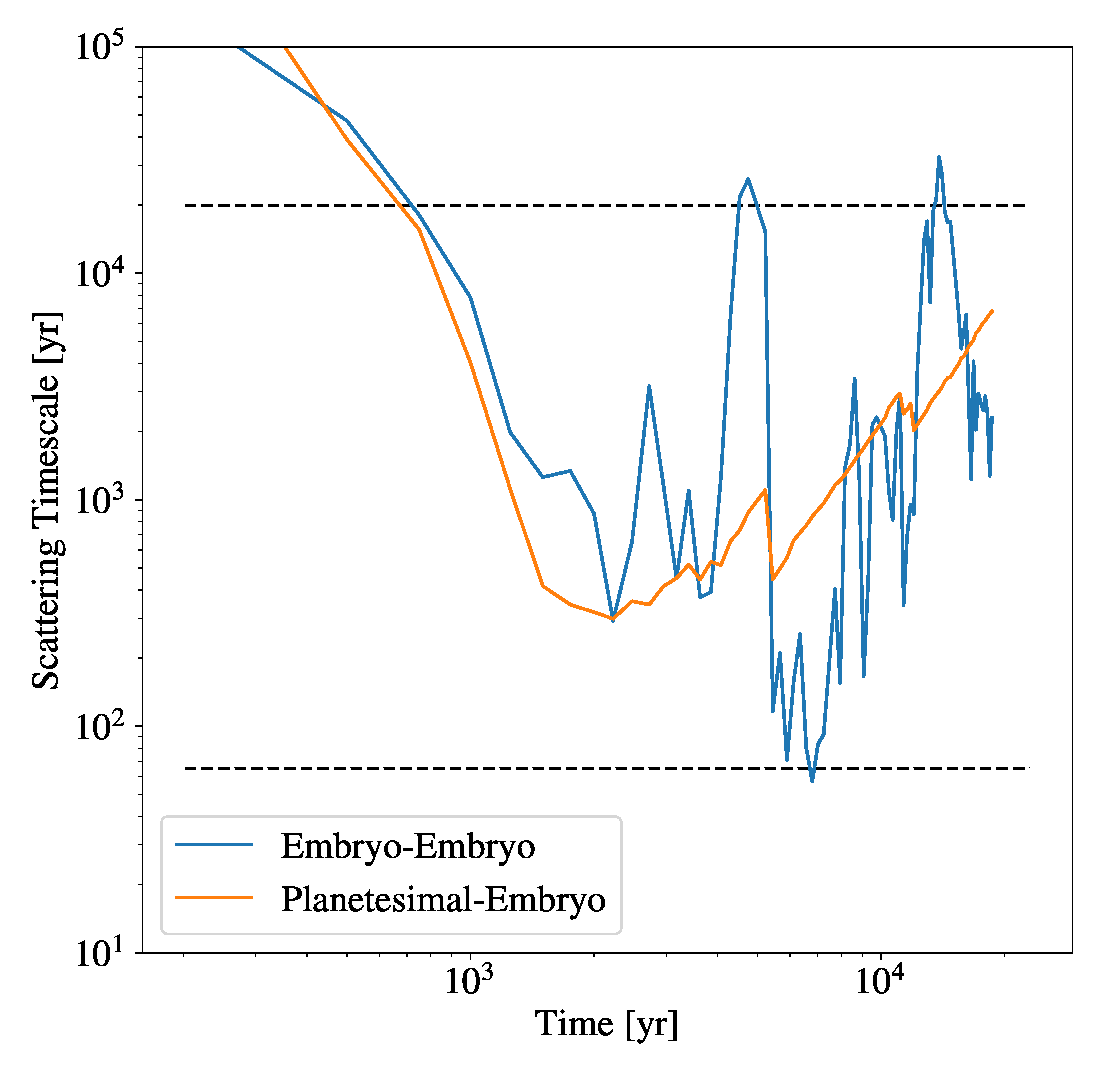
\includegraphics[width=0.5\columnwidth]{figures/plSS/scatter_timescale.eps}
    \caption{The mean scattering time-scale for embryo-embryo (blue curve) and planetesimal-embryo (orange curve) interactions 
    over the course of the high resolution growth simulation. The dashed lines correspond to the simulation time-scale (upper) and 
    longest relevant mean motion resonance time-scale (lower), which is set by the 65:64 resonance.}
    \label{fig:scatter_timescale}
    \end{centering}
\end{figure}

In order for this effect to work, the bodies must keep a constant semi-major axis long enough for resonant interactions to play 
out, while still moving by an appreciable amount over the course of the simulation. The strong scattering time-scale for embryo-embryo interactions and planetesimal-embryo interactions is shown in Figure \ref{fig:scatter_timescale}. This is the timescale 
over which bodies of mass $m$ moving with speed $v$ relative to the local Keplerian velocity will approach each other with an 
impact parameter $b \leq G m / v^{2}$. This is sufficient to cause a large deflection and effectively randomize the orbital 
elements of the bodies. In both cases, the average time between scattering events falls between the longest resonance timescale (set by the 65:64 resonance) and the growth time-scale (set by the duration of the simulation). This indicates that the 
scattering is vigorous enough to occur many times over the course of the simulation, while still being slow enough to allow mean 
motion resonances to act. The strong scattering rate is given by

\begin{equation}\label{eq:scatter}
\dot{\overline{N}} \approx \frac{\Sigma}{m} \Omega_{p} R_{h}^2 \left( \frac{v_{h}}{v} \right)^{4},
\end{equation}

\noindent \cite{murrayclay06} where $\Sigma$ and $m$ are the surface density and individual masses of the bodies being 
scattered, $\Omega_{p}$ is the orbital angular velocity of the bodies and $R_{h}$ and $v_{h}$ are the Hill radius and Hill velocity 
of the object doing the scattering.

As discussed in section \ref{sec:lowvshigh}, viscous stirring plays an important role in the dynamical evolution of the 
planetesimals. The effects of viscous stirring are realized over many weak ($b \gg G m / v^{2}$) but frequent encounters. For a 
population of equal mass planetesimals, the timescale for viscous stirring is given by \cite{ida93}

\begin{equation}\label{eq:vs_timescale}
    \tau_{vs}  = \frac{\left< e^2 \right>}{d \left< e^2 \right> / dt} \approx \frac{1}{40}\left(\frac{\Omega^{2} a^{3}}{2 G m}\right)^{2} \frac{4 m \langle e^{2} \rangle^{2}}{\Sigma a^{2} \Omega},
\end{equation}

\noindent where $a$ and $e$ are the semi-major axes and eccentricities of the individual planetesimals. By using the properties 
of the planetesimal disk at the beginning of simulation (i) in equation \ref{eq:vs_timescale}, we find that the viscous stirring 
timescale is approximately 1000 years. This timescale can be taken as a lower limit because the eccentricity dispersion grows 
over time.

We also briefly consider the importance of planetesimal-driven migration. This is the coherent change in the semi-major axis of 
an oligarch due to repeated weak encounters with planetesimals. An upper limit on the planetesimal-driven migration rate of an 
oligarch is given by \cite{ida00}

\begin{equation}\label{eq:mig}
    \left| \frac{d a}{d t} \right| = \frac{a}{T} \frac{4 \pi \Sigma a^{2}}{M_{*}},
\end{equation}

\noindent where $a$ is the semi-major axis of the oligarch, $T$ is the orbital period of the oligarch and $\Sigma$ is the local 
surface density of the planetesimal disk. For an oligarch on a 1 AU orbit in a planetesimal disk with $\Sigma$ = 10 g cm$^{-2}$, 
the maximum migration rate is roughly $10^{-5}$ AU / yr. \cite{kirsh09} showed that this migration rate is greatly reduced for 
planetesimals whose encounters are dispersion dominated. In simulation (i), the Hill eccentricity of the smallest planetesimals at 
the onset of oligarchic growth is larger than 10, in which case the migration rate is reduced by a factor of at least 100 (see figure 
7 of \cite{kirsh09}). At this rate, it would take an oligarch roughly 1000 years to migrate by a single resonance width ($10^{-4}$ 
AU). This is much longer than the resonance timescale and therefore we do not expect that planetesimal-driven migration would 
disrupt the resonant configuration.

From these results, we conclude that the two simultaneous modes of growth are driven by a difference in the way that loosely 
and densely packed populations of planetesimals exert dynamical friction on large bodies. In the tightly packed case, energy 
transfer between the oligarchs and planetesimals is facilitated by mean motion resonances with the largest bodies.

\begin{figure*}
    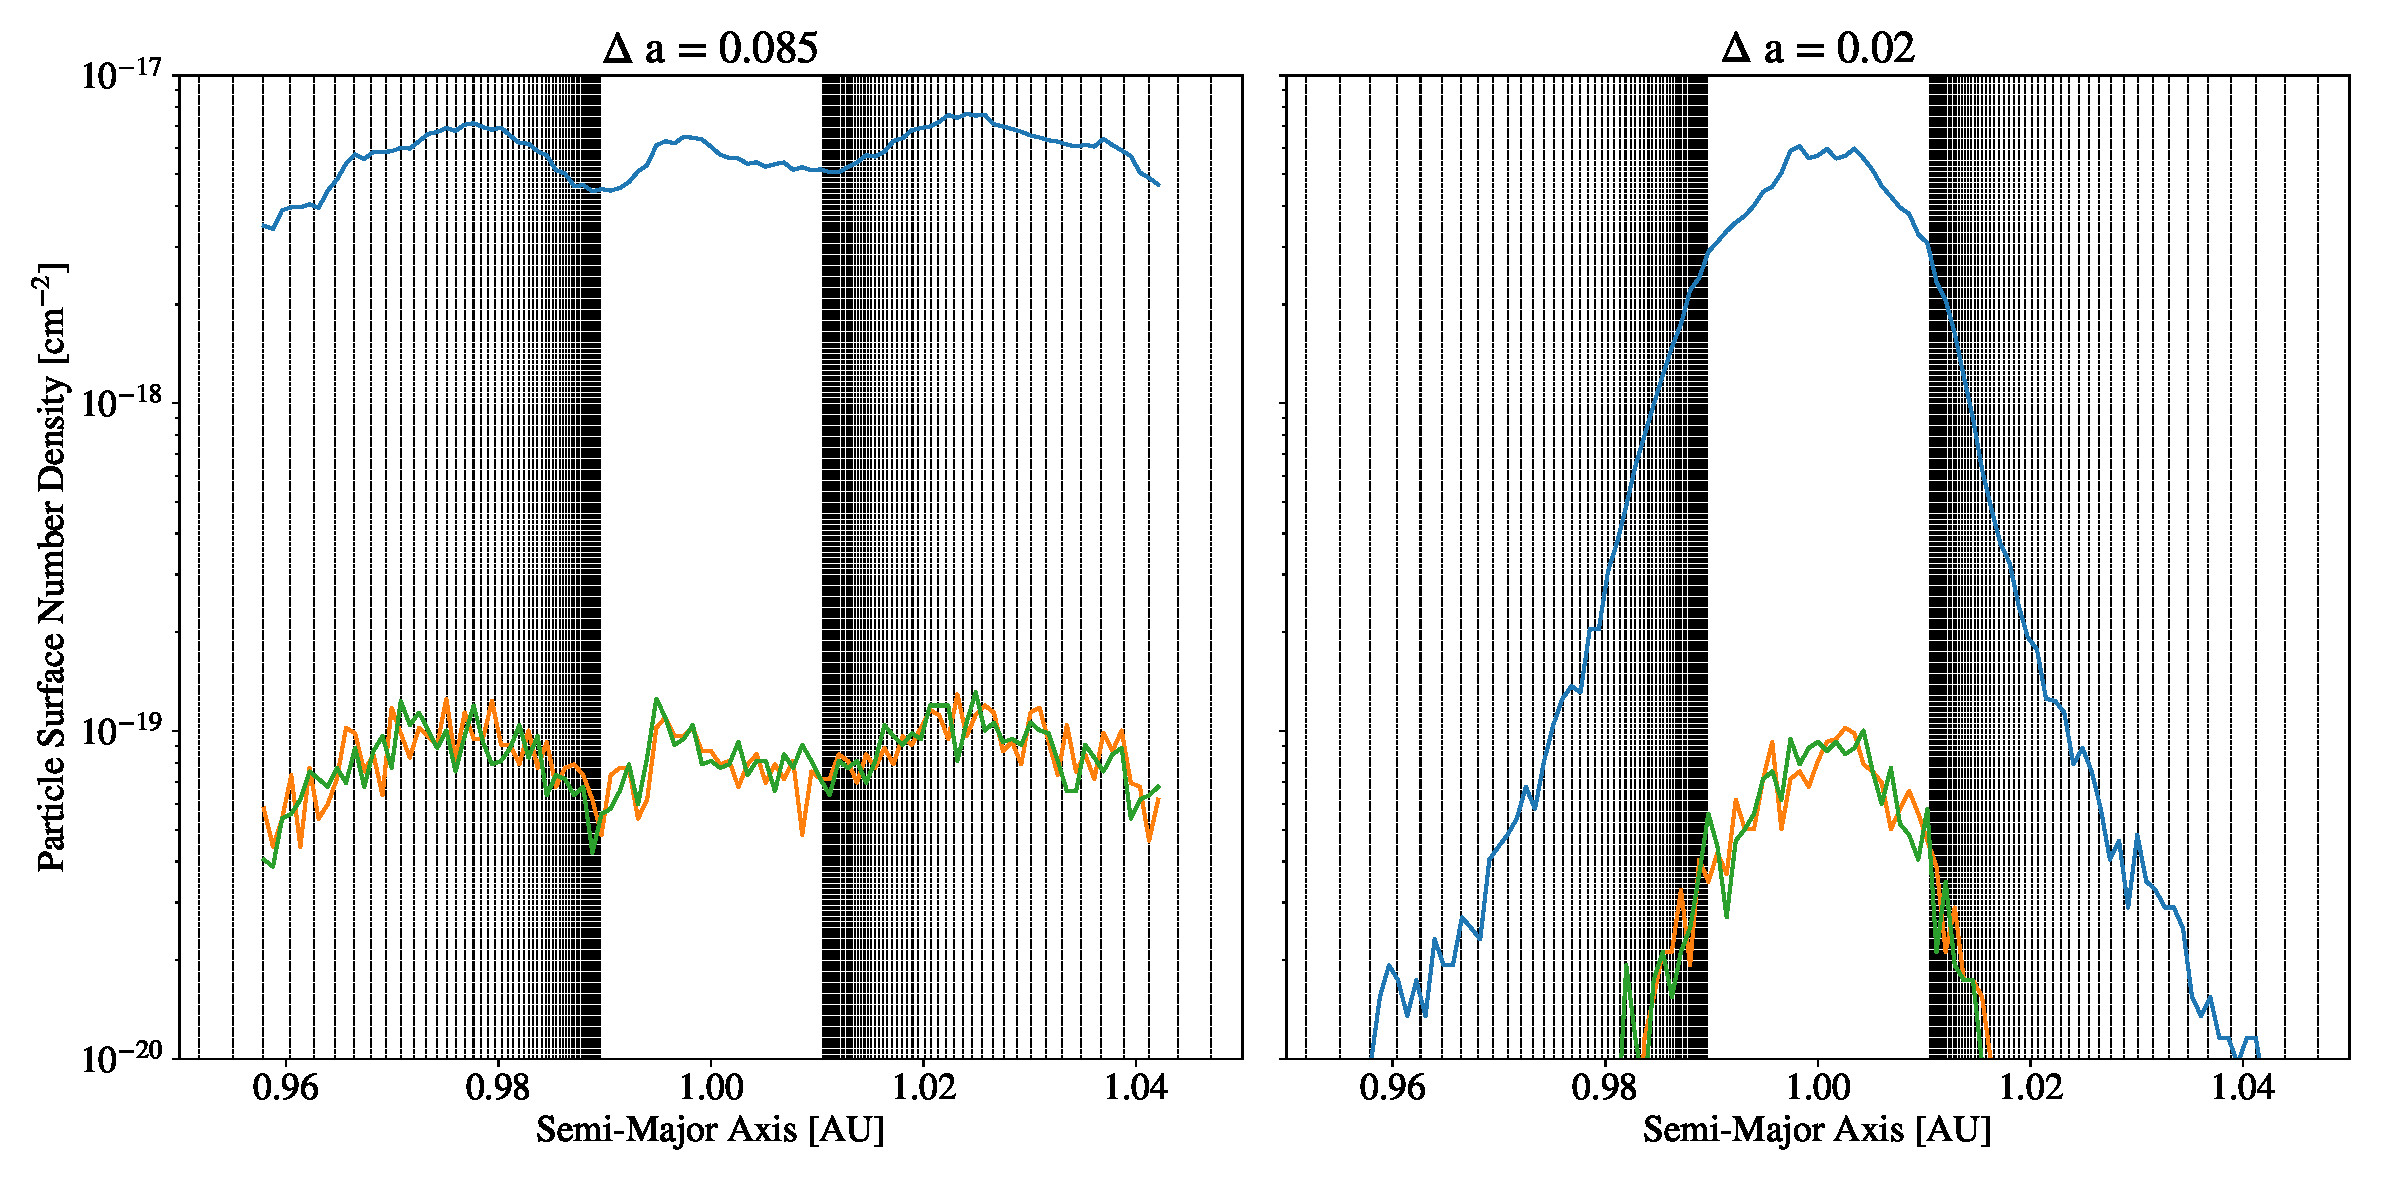
\includegraphics[width=1.0\textwidth]{figures/plSS/surf_den_dyn_fric.eps}
    \caption{Number density profiles of the planetesimals at the end of the $e_{hi}$ (left) and $e_{narrow}$ simulations (right). 
    The blue curves represent the number density of planetesimals less massive than the resonance heating mass ($2 \times 
    10^{22}$ g) and the orange curves represent the number density of planetesimals above this mass. The green curves show 
    the surface number density of planetesimals randomly drawn from the low mass bin, such that the total number of bodies 
    matches that of the high mass bin. The vertical lines indicate the positions of first order mean motion resonances with an 
    embryo at 1 AU.}
    \label{fig:num_den}
\end{figure*}

\subsection{Collisionless Dynamics}\label{sec:dynint}

So far, the most compelling evidence of the resonance heating effect that we have shown is the power law break in the surface 
density distribution in the bottom right panel of Figure \ref{fig:ecc_den_evo}. Because the surface density depends on both the 
mass distribution and spatial distribution of the planetesimals, it is difficult to tell whether the power law break is caused by 
resonances moving the planetesimals around or is simply set by the mass distribution. To clear up this ambiguity, we ran an 
additional set of simulations in which a large planetary embryo is embedded in an annulus of planetesimals, this time ignoring 
the effects of collisions. This forces the mass distribution to be static.

The initial conditions for these simulations were taken from intermediate snapshots from the runs described in section 
\ref{sec:plSS_results}. Specifically, the initial conditions are taken from the end of the runaway growth phase, which correspond to the 
snapshots shown in the top row of Figure \ref{fig:mass_spectrum_evo}. Additionally, a planetary embryo is placed in the center of 
the annulus at 1 AU with an eccentricity of 0.02 and an inclination of 0.01. The mass of the embryo is set at $M = 10^{26}$ g, 
which is approximately the mass of the largest oligarch at the end of the high resolution simulation. Because collisions are 
ignored, \textbf{bodies are allowed to pass through each other and} close encounters are handled with a gravitational softening parameter, the length of which is set to \textbf{what would have been} the physical radius 
of the planetesimals. Both runs are integrated for 2,000 years with fixed timesteps of 0.0025 years. We will refer to the 
collisionless versions of these simulations as $e_{low}$ and $e_{hi}$, respectively. To further demonstrate that the dynamical 
excitation of the small planetesimals is driven by mean motion resonances, we also ran a high resolution collisionless simulation 
with planetesimals outside of the $a$ = 0.99 to 1.01 AU range excluded. We will refer to this simulation as $e_{narrow}$.

As we saw previously, the resonance heating effect manifests itself as an increase in the spacing of the low mass planetesimals. 
Figure \ref{fig:num_den} shows the planetesimal surface number density at the end of the $e_{hi}$ (left) and $e_{narrow}$ (right) 
simulations described above. The vertical dashed lines indicate the locations of the non-overlapping first order mean motion 
resonances with the embryo. The blue curves show the number density of planetesimals below the resonance heating mass, 
which is $2 \times 10^{22}$ g in this case. The orange curves show the number density of planetesimals above this mass. 
Finally, to demonstrate that the difference in dynamical behavior between the low and high mass planetesimals is a population 
effect, the green curve shows the number density of a subsample of planetesimals randomly drawn from the low mass group, 
such that the total number of planetesimals in the subsample matches that of the high mass group.

In both cases, the particle number density is slightly enhanced around 1 AU, which is due to bodies trapped in the corotation 
resonance with the embryo. For the wide annulus, the surface number density decreases and then begins to increase again 
approximately 0.01 AU away from the embryo. As is evident in the left panel of Figure \ref{fig:num_den}, the location at which the 
number density begins to increase corresponds to the location of the closest non-overlapping (j $<$ 65) mean motion 
resonances. Due to conservation of the Jacobi energy (see equation \ref{eq:tiss}), interior MMRs will push bodies inward, while 
exterior resonances move bodies outward. This effect was also observed by \cite{richardson00} (see model B) in that the 
density decreases to the right of interior resonances and increases to the left. Because our setup contains many closely spaced 
resonances, the cumulative effect is that the density smoothly increases as one moves through the resonances. 

Hence, the number density distribution acquires a `W' shape around the embryo, with the low points corresponding to the inner 
edges of the resonant regions. An inspection of the earlier snapshots from this simulation shows that the 'W' structure becomes 
deeper and narrower with time. This is consistent with our resonance heating argument because the resonance time-scale 
decreases as one moves away from the embryo. The stronger, closer resonances become effective last, causing the profile to 
deepen and narrow with time.

The strength of the resonance heating effect depends on the number density of bodies outside of the $0.99 < a < 1.01$ AU 
region, where the resonances are not overlapping. The `W' shaped structure relative to the noise of the high mass (orange) and 
subsampled population (green) is weak compared to the low mass population (blue) due to the fact that there simply aren't many 
bodies sitting within the resonances. This structure is entirely absent from the narrow annulus, shown in the right hand panel of 
Figure \ref{fig:num_den} because the planetesimal number density near the resonances is too low. We infer that this decrease in 
number density of the low mass bodies adjacent to the embryo must also be present in the high resolution growth simulation and 
is enhancing the collision rate below the resonance heating mass.

We also examine the eccentricity evolution of the planetary embryo in the three collisionless simulations, shown in figure 
\ref{fig:e_oli_evo}. A decrease in the eccentricity of the embryo indicates that energy is being lost to the planetesimals. A steeper 
drop in eccentricity implies that the exchange happens more quickly and that the effects of dynamical friction are stronger. Only 
when the resonances are properly resolved and populated does the exchange appear to happen quickly. In both the $e_{narrow}
$ and $e_{low}$ simulations, the decrease in eccentricity of the embryo is gradual. This implies that dynamical friction is stronger 
and energy and angular momentum exchange between the oligarchs and planetesimals proceeds faster when the mean motion 
resonance heating is effective. In the $e_{hi}$ simulation, the eccentricity of the embryo begins to drop more steeply after about 
1000 years. This effect is also noticeable for the $e_{narrow}$ simulation, although it happens sooner. Because we are suddenly 
dropping a massive body into the annulus of planetesimals, the system likely requires some time to return to a state of quasi-
equilibrium. The two-body relaxation time, which is well-described by the viscous stirring timescale \cite{ida93} appears to 
roughly coincide with the change in slope for each of the curves in Figure \ref{fig:e_oli_evo}, although the connection between the 
relaxation of the planetesimals and the eccentricity evolution of the oligarch is not immediately clear. In the $e_{low}$ simulation, 
the change in slope may not be visible due to the fact that the two-body relaxation time is nearly instantaneous due to the small particle count (the relaxation time scales as $N / \ln N$).

\begin{figure}
    \begin{centering}
    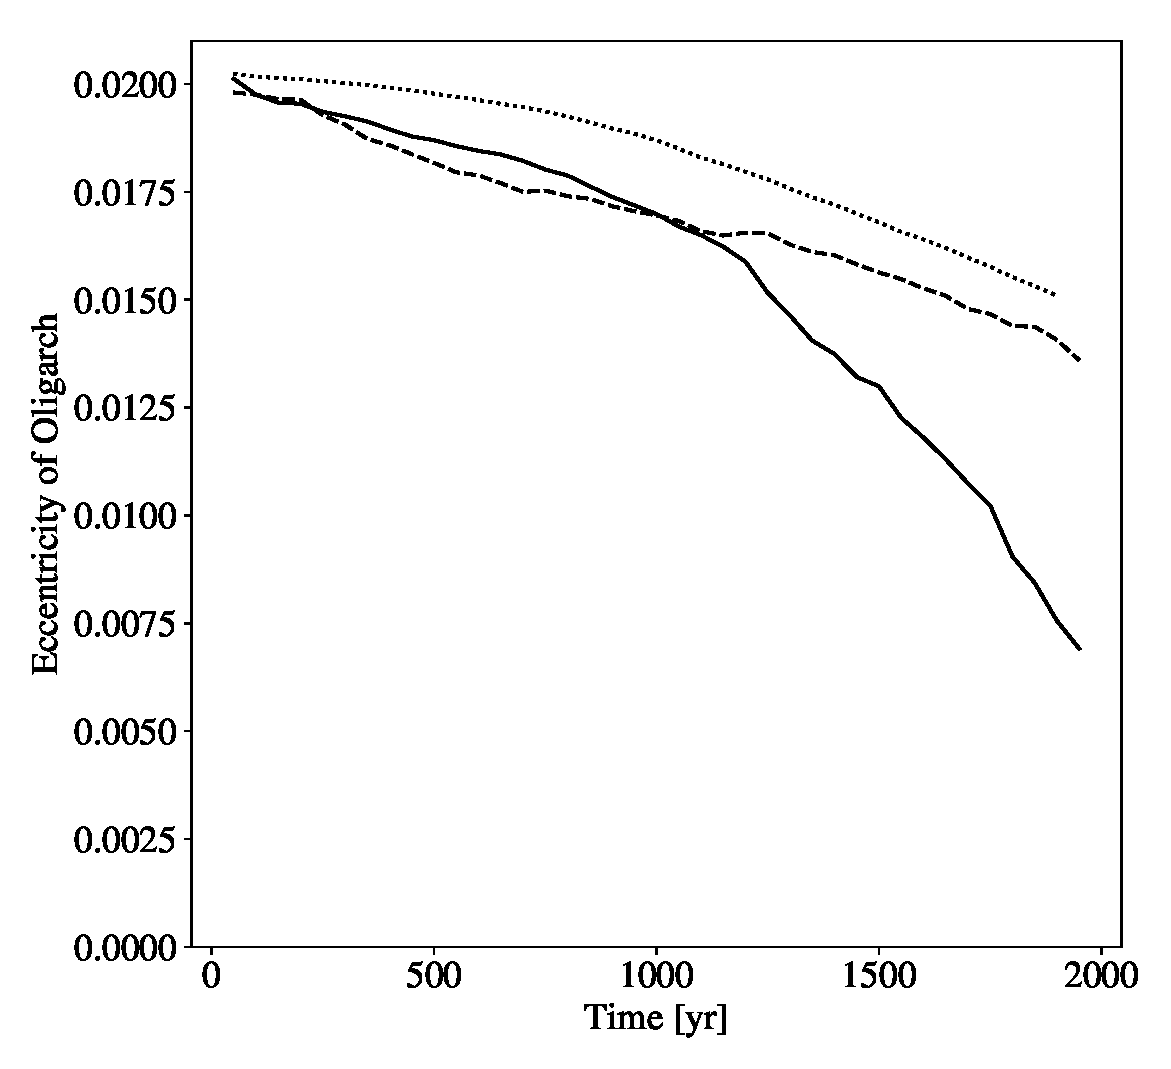
\includegraphics[width=0.5\columnwidth]{figures/plSS/hetero_e_oli.eps}
    \caption{Time evolution of the eccentricity of the oligarch in the $e_{hi}$ (solid), $e_{narrow}$ (dotted) and $e_{low}$ (dashed) 
    simulation.}
    \label{fig:e_oli_evo}
    \end{centering}
\end{figure}

To verify the effectiveness of the resonant interactions, we next examine the evolution of the resonant arguments. The libration 
frequency of a planetesimal in resonance with an embryo is given by \cite{murray00}

\begin{equation}\label{eq:lib_period}
    \omega_{0}^{2} = -3 j_{2}^{2} C_{r} n e^{\left| j_{4} \right|},
\end{equation}

\noindent where $j_{2}$ = -15 and $j_{4}$ = -1 for the 15:14 MMR and $n = \sqrt{G M_{*} / a^{3}}$ is the mean motion of the 
planetesimal. For a planetesimal with a typical eccentricity of $10^{-3}$ inside the 15:14 mean motion resonance with a 
$10^{26}$ g embryo, the libration period is approximately 1000 years. For this reason, it is likely that a particle will undergo only 
a partial libration cycle before being removed from the resonance by two-body scattering. This makes it difficult to verify the 
resonant interaction by searching for libration, rather than circulation of the resonant arguments. However, this also implies that 
the resonances will cause permanent changes to the energy and angular momentum of the planetesimals. In canonical 
perturbation theory, the action conjugate to the resonant argument should evolve secularly because there is a near-constant 
term in the partial derivative of the Hamiltonian with respect to the resonant angle. If the viscous stirring timescale, which is the 
mechanism responsible for the removal of planetesimals from resonance is short compared to the libration period, this secular 
interaction produces a permanent change in the action (and therefore the energy and angular momentum) of a planetesimal 
(see the text following equation 10 in \cite{weinberg07a} for a further discussion of this).

The typical change in the resonant arguments of the planetesimals from the $e_{hi}$ simulation over multiple synodic periods is 
shown in Figure \ref{fig:lib_arg}. The resonant argument is given by \cite{murray00}


\begin{equation}\label{eq:res_arg}
    \phi = j_{1} \lambda_{e} + j_{2} \lambda_{p} + j_{4} \varpi_{p},
\end{equation} 

\noindent where $j_{1} = 15$, $j_{2} = 14$ and $j_{4} = 1$ for the 15:14 MMR. $\lambda_{e}$ and $\lambda_{p}$ are the mean longitudes 
of the embryo and planetesimal, respectively and $\varpi_{p}$ is the longitude of pericenter of the planetesimal. The $\Delta 
\phi$ shown in Figure \ref{fig:lib_arg} is the change in this resonant argument between t=1500 and t=1550 years, well after the 
system has relaxed back to a state of quasi-equilibirum. The blue diagonal lines represent the change in the resonant argument 
due to the Keplerian shearing of the disc. This quantity is derived by taking the time derivative of equation \ref{eq:res_arg},  
which is given by

\begin{equation}\label{eq:res_arg1}
    \frac{d \phi}{dt} = j_{1} \left( \frac{d \varpi_{e}}{dt} + \frac{d M_{e}}{dt} \right) + j_{2} \left( \frac{d \varpi_{p}}{dt} + \frac{d M_{p}}{dt} \right) + j_{4} \frac{d \varpi_{p}}{dt}.
\end{equation} Only the mean anomaly $M = n t$ changes due to the Keplerian shear and so

\begin{equation}
    \Delta \phi_{Kepler} = \sqrt{G M_{*}} \left( j_{1} a_{e}^{-3/2} + j_{2} a_{p}^{-3/2} \right) \Delta t,
\end{equation} where $\Delta t$ is the time interval that we are considering. Note that at the nominal resonance location, $\Delta \phi_{Kepler} = 0$.

\begin{figure}
    \begin{centering}
    \includegraphics[width=0.5\columnwidth]{figures/plSS/lib_arg.eps}
    \caption{The change in the resonant argument for the oligarch and planetesimals near the 15:14 MMR over a 50 year time 
    interval from the $e_{hi}$ simulation. The solid vertical line designates the nominal resonance location and the dashed vertical 
    lines indicate the minimum libration width. The diagonal blue lines represent the change in $\phi$ due to the Keplerian shear 
    of the disc, which is calculated analytically.}
    \label{fig:lib_arg}
    \end{centering}
\end{figure}

Over a 50 year time interval, which is approximately 3 times longer than the synodic period with the embryo, the change in the 
resonant arguments of the planetesimals appear to be dominated by the differential rotation of the disc. Near the nominal 
resonance location, the change in $\phi$ is small. The fact that many planetesimals remain within the resonance width and 
undergo only small changes in $\phi$ over multiple synodic periods demonstrates that the resonant interaction between the 
planetesimals and the embryo is able to proceed. Because the libration period is not short compared to the scattering timescale, 
the resonant interactions will cause permanent changes to the energy and angular momentum of the planetesimals.

\section{Implications of Simplifying Assumptions}\label{sec:assumptions}

\subsection{Gas Drag}

Although the effects of gas drag are weak during the planetesimal accretion stage, we will briefly consider its effect to ensure 
that it would not alter or remove the $10^{22}$ g bump. One way to describe the importance of gas drag on a planetesimal is 
with the stopping time \cite{adachi76}. In the Stokes regime, where the mean free path of gas particles is much smaller than the 
radius of the planetesimals ($\lambda \ll$ s), the stopping time is given by

\begin{equation}\label{eq:t_stop}
    t_{s} = \frac{2 m}{C_{D} \pi s^{2} \rho_{g} v}.
\end{equation}

\noindent Here, $\rho_{g}$ is the local density of the gas and $C_{D}$ is the drag force coefficient, which is of order unity in this 
regime. The gas density of the solar nebula is approximately $2 \times 10^{-9}$ g cm$^{-3}$ at 1 AU \cite{hayashi81}.

The relative velocity between the planetesimals and the gas is set by both the random motions of the planetesimals and the fact 
that the gas orbits at a sub-Keplerian speed due to its internal pressure support. The planetesimal velocity due to random 
motions is given by \cite{lissauer93}

\begin{equation}\label{eq:vrnd}
    v_{rnd} = v_{k} \sqrt{\left< e^2\right> + \left< i^2\right>}.
\end{equation}

\noindent At the beginning of the simulation (i), $v_{rnd}$ is on the order of $10^3$ cm s$^{-1}$. The headwind speed due to the 
sub-Keplerian motion of the gas is given by \cite{adachi76}

\begin{equation}\label{eq:vgas}
    v_{gas} = v_{k} \left( 1 - (1 - 2 \eta)^{1/2} \right),
\end{equation}

\noindent \textbf{where $\eta$ is a dimensionless parameter that describes the strength of the headwind.} At 1 AU in the solar nebula, $\eta \approx$ 0.002, which gives $v_{gas} \approx$ 6000 cm s$^{-1}$. From equation 
\ref{eq:t_stop}, the smallest planetesimals in simulation (i) have a stopping time on the order of $10^4$ years. This is much 
longer than the synodic period of the relevant planetesimal-oligarch resonances, therefore we expect the dynamics of even the 
smallest planetesimals to be entirely dominated by the resonances.

Additionally, gas drag can drive the inward radial drift of small bodies. Although the relatively large stopping time of the 
planetesimals suggests that this effect should be unimportant, the resonances are narrow enough that even a small amount of 
radial drift could quickly remove planetesimals from their influence. The radial drift velocity of a particle is given by 
\cite{weidenschilling77}

\begin{equation}\label{eq:v_drift}
    v_{r}  = -\frac{2 v_{gas}}{\Omega t_{s} + \left( \Omega t_{s} \right)^{-1}}.
\end{equation}

\noindent where $\Omega$ is the orbital angular frequency of the body being considered. Using the values for $v_{gas}$ and 
$t_{s}$ described above, the inward radial drift speed of the smallest planetesimals is 0.1 cm s$^{-1}$. At this rate, a 
planetesimal will drift across a typical resonance width ($10^{-4}$ AU) in about 1000 years. This is comparable to the viscous 
stirring timescale, which suggests that radial drift should not have a significant effect on the resonant dynamics.

Massive bodies can create density waves in the gas disk which carry away angular momentum \cite{goldreich79, goldreich80} 
through an effect known as type I migration (for a recent review see \cite{baruteau14}). The strength of this effect scales linearly 
with the mass of the body and should therefore be most effective for planetary embryos. In addition to gas drag causing 
planetesimals to radially drift across resonances, type I migration can cause planetary embryos to drift inwards, potentially 
moving the resonances before they have a chance to act on the planetesimals. \cite{tanaka02} provides an analytic expression 
for the torque exerted on a body embedded in a three-dimensional gaseous isothermal disk as

\begin{equation}\label{eq:t1mig_torque}
     \Gamma = -\left( 1.364 + 0.541 \alpha \right) \left (\frac{m}{M_{*}} \right)^{2} \left( \frac{r \Omega}{c_{s}} \right)^{2} \Sigma r^{4} \Omega^{2},
\end{equation}

\noindent where $\alpha$ is the power law index of the radial surface mass density profile $\Sigma \propto r^{-\alpha}$ of the gas 
and $c_{s}$ is the local sound speed of the gas, $m$ is the mass of the body, $\Omega$ is the orbital angular frequency of the 
body and $r$ is the orbital distance of the body. The radial migration velocity is given by

\begin{equation}\label{eq:t1mig_rate}
    \dot{r} = \frac{-2 r \Gamma}{L},
\end{equation}

\noindent where $L = m \left( G M_{*} r \right)^{1/2}$ is the total angular momentum of the body. For a $10^{26}$ g embryo 
orbiting at 1 AU and taking $\alpha$ = 3/2, $\Sigma$ = 1700 g cm$^{-2}$ and $c_{s}$ = $10^{5}$ cm s$^{-1}$ \cite{hayashi81}, 
the inward migration speed is $2 \times 10^{-7}$ AU yr$^{-1}$. At this rate, the 15:14 MMR with an embryo will migrate by a 
entire resonance width in roughly 500 years, which is much longer than the synodic period. It should be noted that the analysis 
of \cite{tanaka02} has been shown to produce migration rates that are up to a factor of $10^{3}$ too large to be consistent with 
observed populations of exoplanets \cite{ida04, alibert05, miguel11}. The migration timescale derived above should therefore 
be taken strictly as a lower limit.

As migration proceeds, planetesimals can have their spatial distribution altered as they become trapped in exterior resonances 
with protoplanets \cite{weidenschilling85}. A necessary condition for resonant trapping to occur is that the drift timescale of a 
planetesimal across a resonance must be much longer than the libration period \cite{dermott88}. As we calculated in section 
\ref{sec:dynint}, a typical libration period is around 1000 years. This is comparable to the timescale for \textbf{two-body} 
scattering and also for radial drift of planetesimals across a resonance due to gas drag. Therefore, we do not expect that exterior 
resonances should be effective at trapping drifting planetesimals.

\subsection{Inflated Collision Cross Section}

As discussed in section \ref{sec:numerical}, enhancing the geometric collision cross section $f$ of the planetesimals by a factor 
of 6 only slightly reduces the effectiveness of gravitational scattering. More importantly, varying $f$ alters the accretion 
timescale. The implication of this is that a longer accretion timescale causes oligarchic growth to commence later when the disk 
is more dynamically excited. The dynamical excitation of the disk, which is set by the rms eccentricity, alters the libration width of 
planetesimals in resonance with the oligarchs. In section \ref{sec:resonances}, we argued that the intersection between the 
libration width and the radial spacing between planetesimals sets the location of the bump in the mass distribution. Because the 
radial spacing between planetesimals increases with mass and the libration width of the resonances gets larger with time, the 
mass of the bump would be larger had we used $f$ = 1.

It is difficult to predict exactly how much $f$ reduces the accretion timescale, but \cite{kokubo96} showed that it is by no more 
than factor of $f^2$. Integrating equation \ref{eq:vs_timescale}, the rms eccentricity scales with $t^{1/4}$. Having enhanced the 
collision cross section by a factor of 6, the rms eccentricity should be a factor of $(f^2)^{1/4} \approx 2.5$ times larger with a 
realistic collision cross section. Using equation \ref{eq:lib_width}, a factor of 2.5 increase in the eccentricity of a planetesimal 
increases the libration width by a factor of about 1.6. Looking at Figure \ref{fig:res_mass}, this would cause an extremely 
insignificant \footnote{The difference in libration width between the 65:64 and 15:14 resonance produces a much larger spread in the exact value of the resonance heating mass.} change in the resonance heating mass.

\subsection{Fragmentation}

Because our model does not include the effects of collisional fragmentation, we examine the statistics of the collisions in 
simulation (i) to estimate its effects had it been included. Here, we find that roughly 60 percent of the collisions occur with a 
relative velocity larger than the mutual escape velocity of the two planetesimals. Assuming that the planetesimals are rubble 
piles with no internal strength, these high velocity collisions should be completely disruptive. Previous studies of planetesimal 
accretion have shown that including the effects of fragmentation tends to slow down the accretion process, but does not 
qualitatively change it \cite{wetherill93, leinhardt05}.

If we separate the collision statistics into those occurring between bodies below the bump mass ($< 10^{22}$ g) and those 
above the bump mass, we do not see a significant difference in the relative amount of catastrophic collisions. Above the bump 
mass, about 60 percent of collisions occur at disruptive velocities, while 70 percent of collisions between bodies below the bump 
mass occur at these high relative velocities. Because we do not have multiple simulations to draw from, it is difficult to estimate 
errors to tell whether this difference is statistically significant.

Assuming that disruptive collisions are not significantly more common below the bump mass, we expect that fragmentation 
would alter our results by lengthening the accretion timescale. As discussed in the previous section, the location of the bump 
depends on the rms eccentricity of the planetesimals during the oligarchic growth phase. If this phase takes longer to 
commence, the libration widths of the resonances would be larger when the embryos form, which increases the mass below 
which the resonant heating is effective. Although it is difficult to determine by exactly how much fragmentation extends the 
accretion timescale, statistical models of planetesimal growth show that $10^{26}$ g embryos can be formed in $10^{5}$ years 
\cite{wetherill93} when the effects of fragmentation are included. We showed in the previous section that a factor of 36 increase 
in the accretion timescale (720,000 years) makes a negligible difference in the location of the bump in the mass spectrum. 
Similarly, we expect that including the effects of fragmentation would make a negligible contribution to the bump mass.

\section{Dependence on Initial Planetesimal Mass}\label{sec:intermed}

In order to demonstrate that our results are robust, and also to gain some insight into how the resonance heating mass is related 
to the initial planetesimal mass, we ran two more simulations of planetesimal growth at intermediate resolutions. Our choice of 
initial planetesimal mass in the high resolution simulation was somewhat arbitrary and understanding how this parameter affects 
the resulting distribution of masses is necessary in order to connect our results with observations of small Solar System bodies.

The configurations used were identical to the high resolution run described in section \ref{sec:ics}, except that the particle count 
was changed. These two additional runs contained 250,000 and 500,000 starting planetesimals, which corresponds to $m = 2.4 
\times 10^{21}$ and $m = 4.8 \times 10^{21}$ g, respectively, at the same surface density. To match the same eccentricity 
dispersion as the models described in section \ref{sec:ics}, we used $\langle e^2 \rangle^{1/2} = 3.17 h/a$ and $\langle e^2 
\rangle^{1/2} = 2.52 h/a$, with the inclination dispersion set to half of those values.

Figure \ref{fig:resolution_mass_dist} shows the mass spectrum at T = 20,000 years in the high resolution growth simulation, 
along with the intermediate resolution growth simulations mentioned above. In all three cases, the bump in the mass distribution 
approximately matches up with the resonance heating mass. There is a clear positive trend between the resonance heating 
mass and the initial planetesimal mass $m$, which we attribute to two things. First, larger planetesimals will be spaced further 
apart for a fixed disc surface density. This pushes the intersection point between the planetesimal spacing and libration width to 
higher mass. Secondly, larger initial planetesimals will cause oligarchic growth to begin at a higher mass \cite{morishima17}. 
This increases the libration width of the resonances, which moves the intersection between planetesimal spacing and resonance 
width to a higher mass.

\begin{figure}
    \begin{centering}
    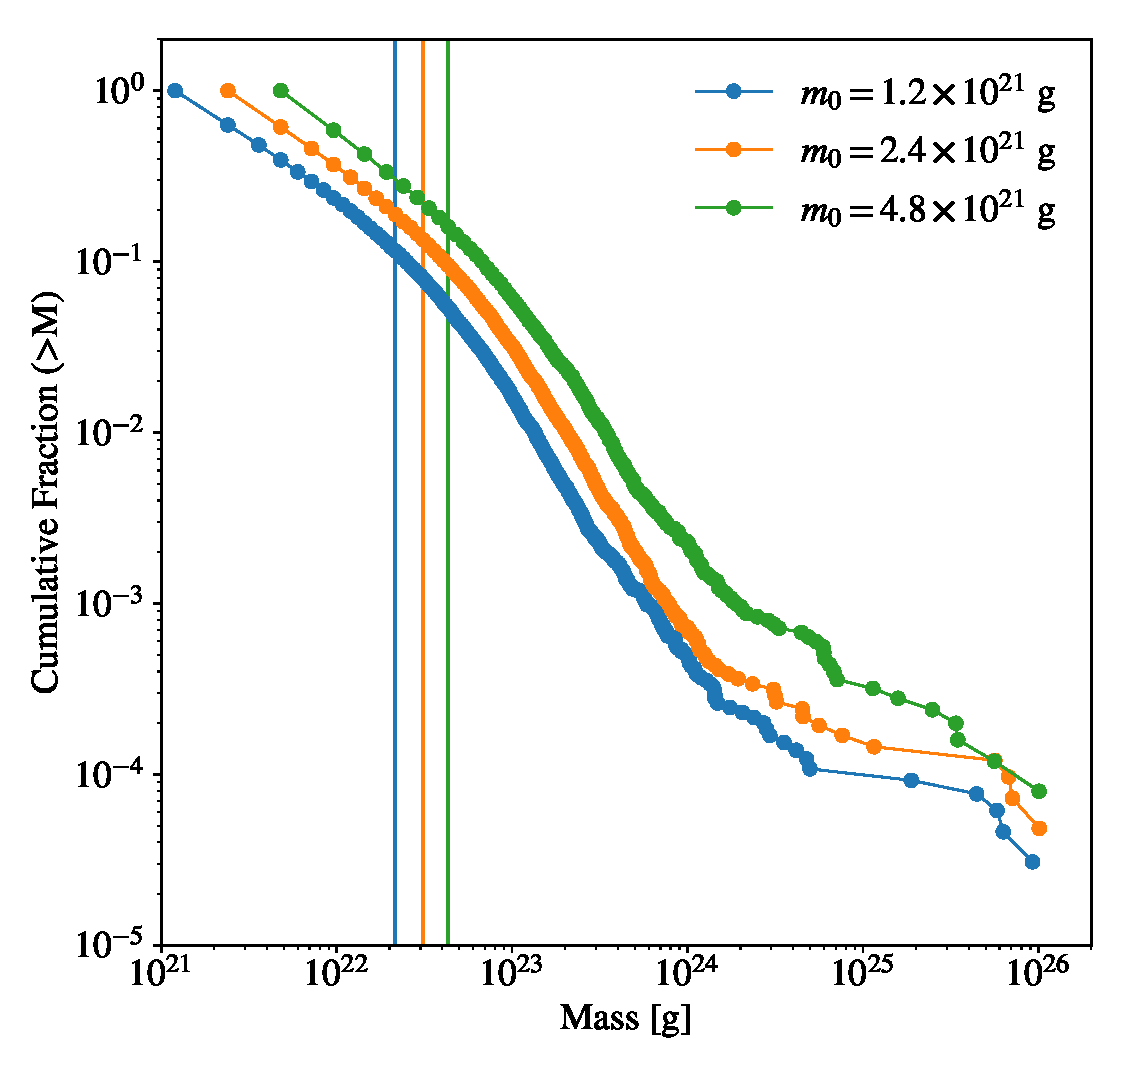
\includegraphics[width=0.5\columnwidth]{figures/plSS/cum_model_comparison.eps}
    \caption{The cumulative mass distribution of planetesimals at the end of the three high-resolution growth simulations. The 
    vertical lines represent the mass at which the planetesimal spacing in semi major axis falls below the libration width of the 
    MMRs.}
    \label{fig:resolution_mass_dist}
    \end{centering}
\end{figure}

The size frequency distribution of asteroid belt objects is known to exhibit a power law break around around 
$1.05 \times 10^{21}$ g \cite{jedicke02}. The fact that the knee in the mass distribution is reproducible and appears sensitive to 
$m_{0}$ demonstrates that this value could be tuned to constrain planetesimal formation models by matching the observed 
mass of the bump with simulations. There is evidence that the shape of the SFD for asteroid belt objects more massive than 
about 100 km reflects that of the primordial population \cite{morbidelli09}. Although the purpose of this chapter is not to try to tune 
the model to match observations, we show the mass distribution from the $N=10^6$ growth simulation alongside the SFD of 
asteroid belt objects \cite{bottke05} in Figure \ref{fig:mass_dist_ast_compare} for comparison. Although the bump location in all 
of our simulations is larger than 100 km, a smaller initial planetesimal mass would probably produce a better match. The slope of 
the mass distribution above the bump mass matches reasonably well in both cases, but the slopes on the low mass end are 
discrepant. As the results from Figure \ref{fig:mass_spectrum_comp} show, a wider annulus tends to produce a shallower slope 
below the resonance heating mass. A better match might be made by simulating a wider annulus which includes resonances 
further from the embryos. Unfortunately, simulating an annulus wide enough to resolve all of the first order MMRs would require 
an extremely large number of particles.

As discussed in section \ref{sec:assumptions}, we do not expect the simplifying assumptions of perfect accretion and the 
absence of gas drag, along with the artificially inflated collision cross section to have a significant effect on the size distribution of 
accreted bodies. Because we have proposed that the initial planetesimal size could be reduced to better match the break in the 
asteroid belt SFD, we briefly consider the smallest sized planetesimals for which the resonant heating effect is not damped by 
gas drag. This will occur when the synodic period of the resonance becomes comparable to the stopping time. The latter quantity 
is given by equation \ref{eq:t_stop} and scales linearly with planetesimal size. For 100 km planetesimals, we showed that the 
stopping time is around $10^4$ years. The stopping time becomes comparable to the synodic period for bodies smaller than a 
few km in size, at which point \textbf{the resonant heating mechanism should no longer operate}.

\section{Summary and Discussion} \label{sec:discussion}

We have revealed a new mode of growth during the planetesimal accretion phase by simulating the interaction between 
oligarchs and planetesimals at unprecedented resolution. Shortly after the onset of oligarchic growth, a bump develops in the 
mass distribution of planetesimals. Below the bump mass, the surface density of planetesimals follows a shallower power law 
distribution. The break occurs near the mass at which the radial spacing of planetesimal matches the libration width of first order 
mean motion resonances with the oligarchs. These resonances, which are preferentially populated by the more numerous low 
mass planetesimals, act as effective pathways for dynamical friction to transfer energy and angular momentum from the 
oligarchs to the planetesimals. This result is analogous to the resolution dependence that \cite{weinberg07a, weinberg07b} 
found when examining the interaction between the bar and halo of a galaxy. This also matches the results of \cite{obrien06} and 
\cite{cionco02}, which showed that finer granularity in a planetesimal disc increases the effectiveness of dynamical friction. 
Bodies below the bump mass, which are packed tightly enough together to populate the resonances receive a disproportionate 
amount of energy and angular momentum from the oligarchs. Because this happens when the disc is hot enough to render 
gravitational focusing ineffective, this enhances the growth of the smallest planetesimals and produces a bend in the mass 
distribution.

Additionally, we ran a high resolution planetesimal growth simulation in which the width of the annulus was limited to exclude 
some of the resonances. Doing so mostly suppressed the formation of the bump near the resonance heating mass, although it 
did not completely get rid of it. We attribute this to the fact that we cannot make the annulus narrow enough to exclude all of the 
important resonances without introducing strong boundary effects which interfere with planetesimal growth. The fact that the 
feature in the mass distribution was greatly diminished when the many of the resonances were excluded is strong evidence that 
the MMRs are responsible for creating this bump.

\begin{figure}
    \begin{centering}
    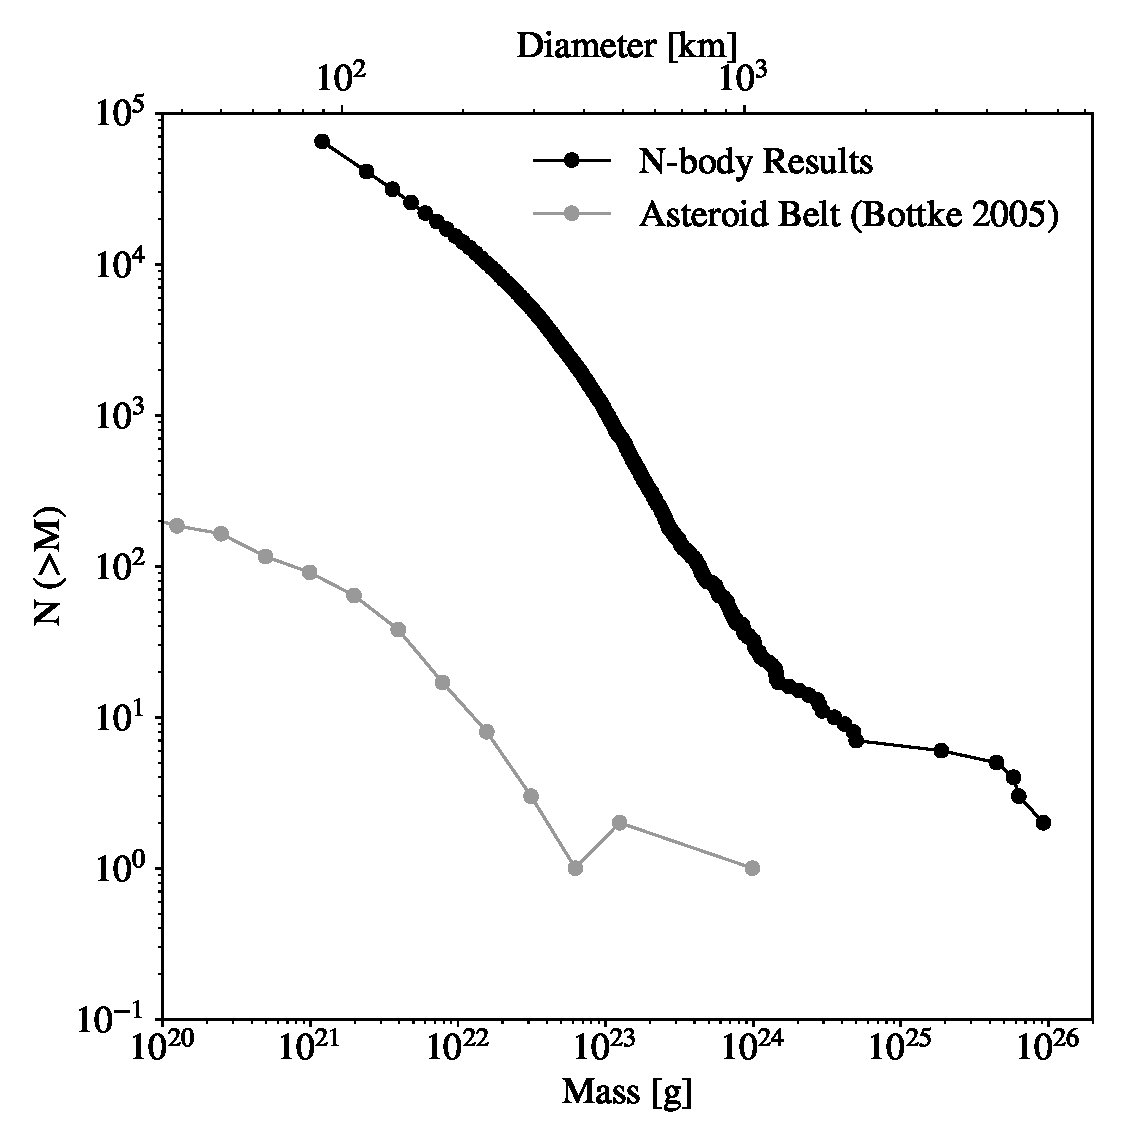
\includegraphics[width=0.5\columnwidth]{figures/plSS/cum_asteroid_comparison.eps}
    \caption{A comparison between the cumulative number of objects in our high resolution growth simulation (black curve) and 
    the present day asteroid belt \cite{bottke05} (gray curve) as a function of size and mass.}
    \label{fig:mass_dist_ast_compare}
    \end{centering}
\end{figure}

We confirmed this dynamical effect by placing a massive oligarch into a smoothly varying distribution of planetesimal masses. 
Within a few thousand orbits, the low mass planetesimals sitting within the zone of influence of the resonances began to migrate 
outwards, leaving a dearth of low mass bodies around the embryo. This effect did not appear when we simulated a similar 
heterogeneous distribution of masses, but limited the width of the annulus to exclude many of the MMRs. Additionally, the 
eccentricity of the oligarch decreased much more quickly when placed in a finely resolved disc with populated MMRs.

This result is significant because it suggests a new potentially observable link between the planetesimal formation process and 
the residual population of planetesimals in the present day Solar System. We showed that the mass distribution in our highest 
resolution simulation looks qualitatively similar to the SFD of objects in the asteroid belt, which, for objects larger than $\approx$ 
100 km, reflects the population of planetesimals at the end of the accretion stage \cite{morbidelli09}. We demonstrated that 
tuning the initial planetesimal mass in our simulation changes the location of the bump. This could potentially be matched with 
the observed 100 km feature in the asteroid belt to constrain planetesimal formation models. Additionally, using a wider annulus, 
which populates more of the first order MMRs, tends to produce a shallower slope on the low mass end of the mass distribution, 
which matches more closely with observations.

As discussed in section \ref{sec:bump}, there are a couple of explanations for this bump feature which were obtained from 
statistical models of planetesimal coagulation. It is unlikely that this resonance heating effect would naturally emerge from a 
statistical growth model unless it was explicitly built in. For this reason, this resonance heating effect has likely not been 
considered before. To our knowledge, no one has ever run an N-body simulation of planetesimal accretion to the oligarchic 
growth phase at this resolution.

Our results show that a feature similar to the power law break in the size distribution of asteroid belt objects can be produced 
without the effects of fragmentation, in contrast to \cite{morbidelli09}. Although our model does not account for the effects of 
fragmentation, the statistics of collisions above and below the bump mass are quite similar. We do not expect that including the 
effects of collisional fragmentation would significantly affect the location or strength of the bump. Regardless, these results 
demonstrate that a careful treatment of the dynamics is necessary to properly model planetesimal accretion during the oligarchic 
growth phase.

\section{Chapter Appendix: Mean Motion Resonance Test}

To demonstrate that {\sc ChaNGa} can properly track the motions of bodies in a mean motion resonance over many orbits, we 
present a test case with a central star, a perturbing massive body and a planetesimal. Although the simulations presented in this 
chapter are far more complex than this three body setup, the resonant interactions that produce the bump in the mass distribution 
are driven by the most massive bodies in the simulation. Because there are only a handful of these massive bodies, the tree 
approximation should have a negligible effect on the force contribution from these objects. For this reason, the behavior shown 
here should also apply to the previously presented simulations of planetesimal growth.

To test that the resonant interaction evolves correctly, we follow the evolution of the planetesimal in the complex x-y plane 
defined by the variable \cite{duncan89}

\begin{equation}\label{eq:complex}
    z = \left(G M_{*} a\right)^{1 / 4}\left\{2\left[1-\left(1-e^{2}\right)^{1 / 2}\right]\right\}^{1 / 2} \exp \left[i(\overline{\omega}-\lambda)\right],
\end{equation}

\noindent where a, e, $\overline{\omega}$ and $\lambda$ are the semi-major axis, eccentricity, longitude of perihelion and mean 
longitude of the planetesimal. If these values are recorded at the moment of opposition between the perturber and the 
planetesimal ($\lambda - \lambda_{p} = \pi$), the trajectory of the planetesimal should trace out a closed loop in the x-y plane. 
This indicates that an approximate Hamiltonian of the system is preserved and the resonant interaction is properly accounted for.

Figure \ref{fig:threebody} shows the evolution of the planetesimal over 20,000 years (about 130 synodic periods) in the complex 
x-y plane. The orbital elements of the planetesimal at the exact moment of opposition are calculated via linear interpolation. The 
perturbing body is placed at 1 AU on a circular orbit and has a mass of $10^{26}$ g, which is similar to the final mass of the 
embryos presented in simulation (i). The planetesimal is given a mass of $1.2 \times 10^{22}$ g and is placed on a coplanar 
orbit with a semi-major axis of 0.95501, which corresponds to the nominal location of the 15:14 mean motion resonance with the 
perturber. To start the planetesimal in a stable equilibirum, its orbital eccentricity is set to $10^{-2}$ so that the longitude of 
pericenter is well-defined. Fixed timesteps of $\Delta$T = 0.0025 yrs are taken, which is the same as the previous simulations. In 
this configuration, the Jacobi constant is small and so the planetesimal follows a circular trajectory in the complex plane. 
Because the perturbing body is on a circular orbit, the forced eccentricity is zero and the trajectory of the planetesimal is 
centered at the origin. Most importantly, trajectory of the planetesimal appears to follow a closed loop, which indicates that an 
approximate Hamiltonian is preserved and the integration is accurate enough to follow mean motion resonances in this 
configuration.

\begin{figure}
    \begin{centering}
    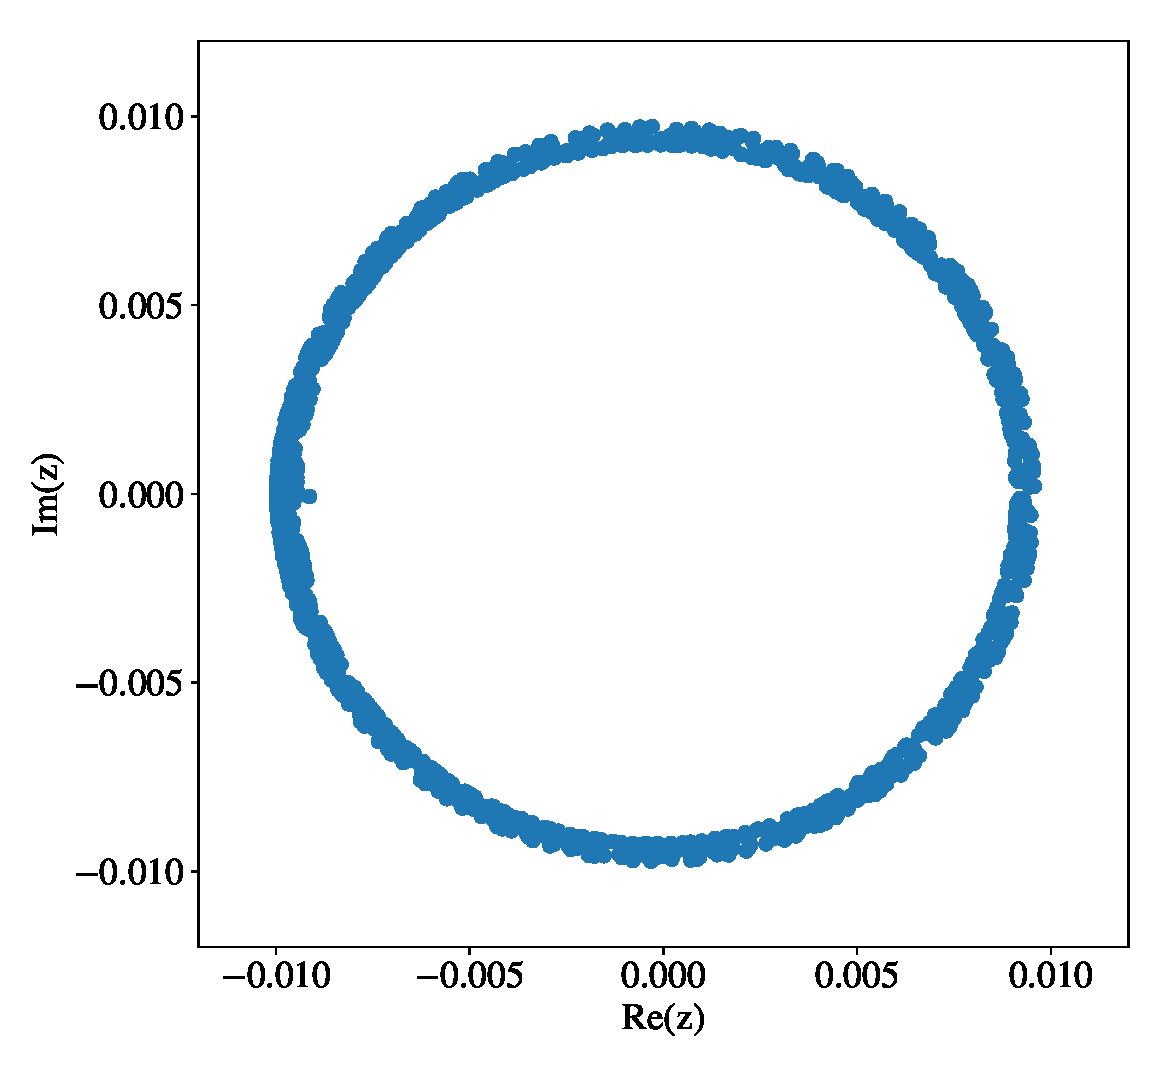
\includegraphics[width=0.5\columnwidth]{figures/plSS/threebody_complex.eps}
    \caption{The evolution of the planetesimal in the complex plane defined by equation \ref{eq:complex}. Each point represents 
    the state of the system when the perturber and planetesimal are at opposition.}
    \label{fig:threebody}
    \end{centering}
\end{figure}

\begin{figure*}
    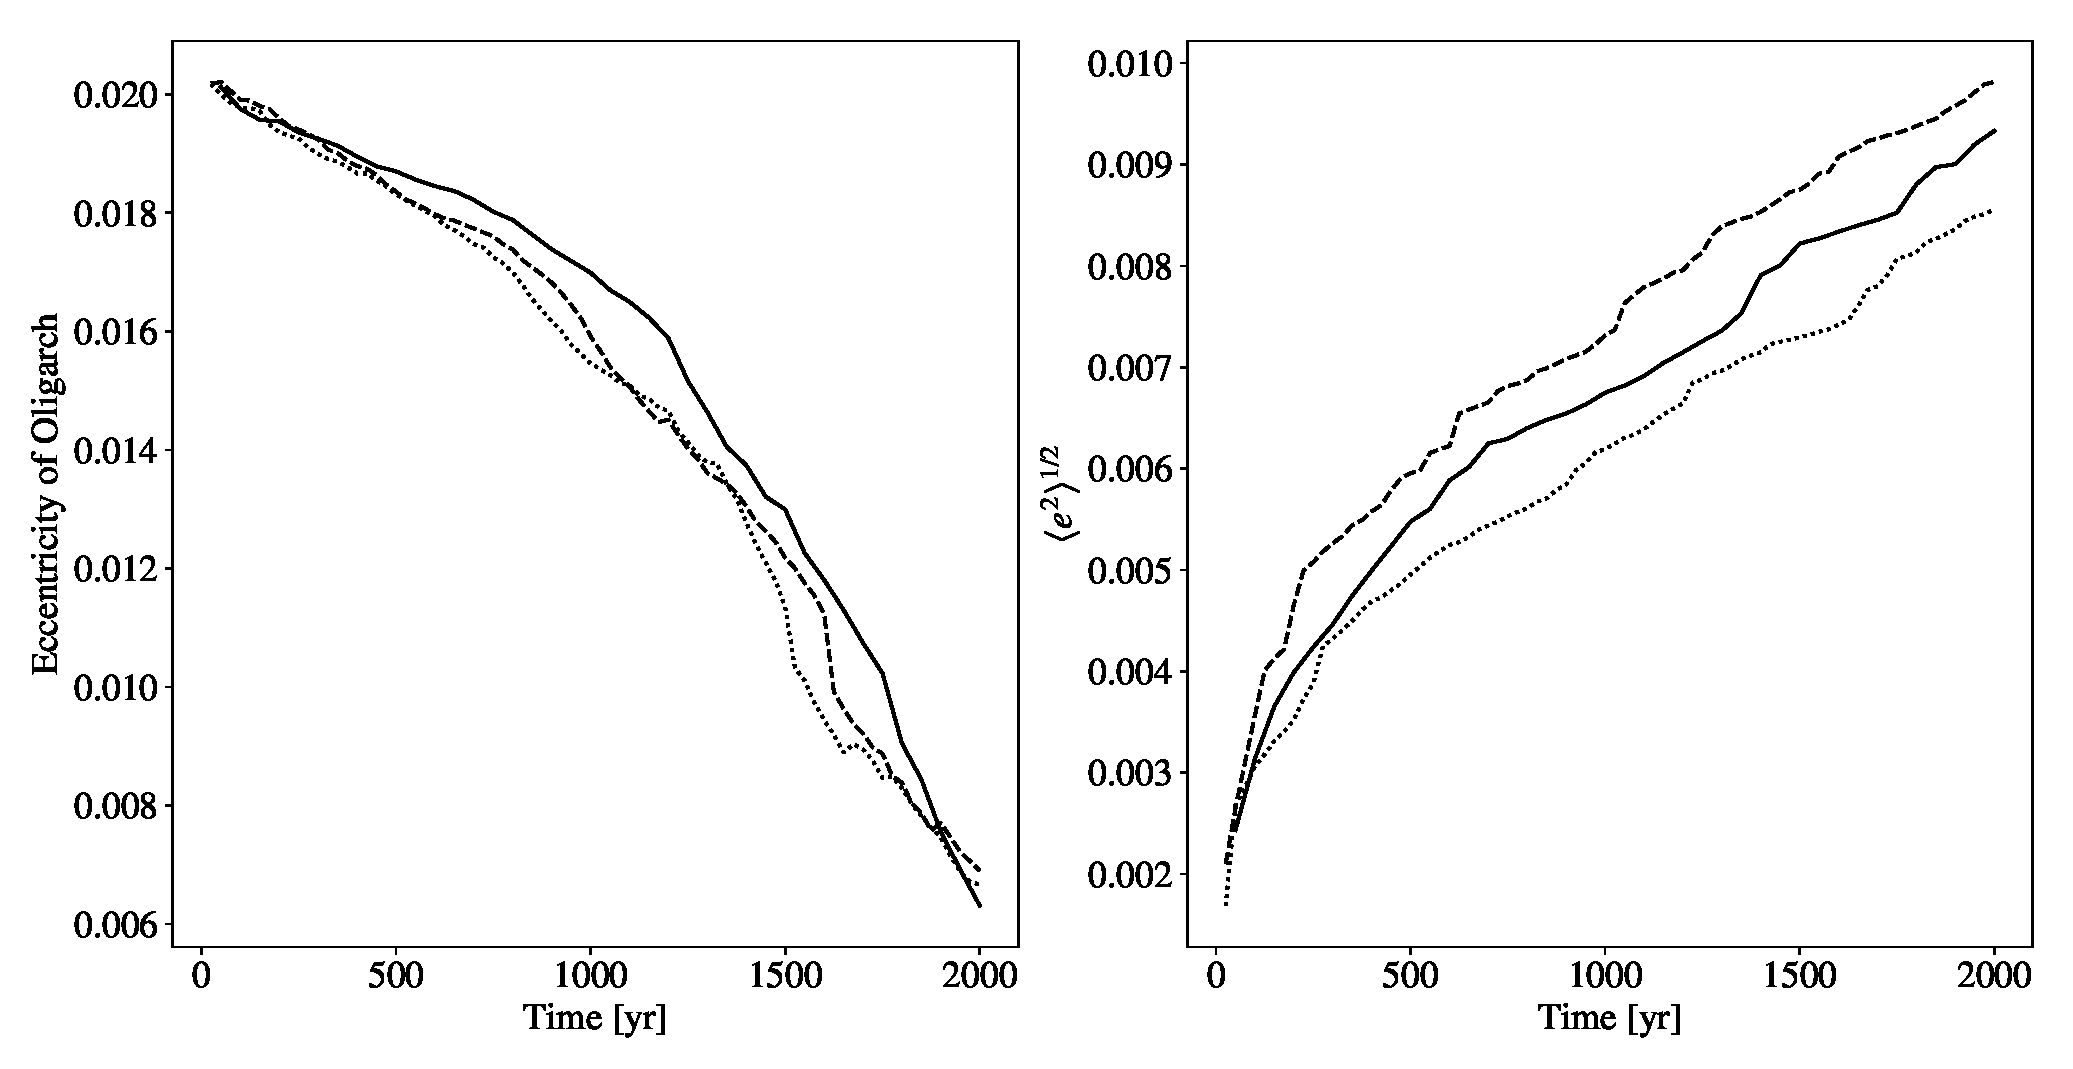
\includegraphics[width=\textwidth]{figures/plSS/theta_test.eps}
    \caption{Time evolution of the eccentricity of the oligarch (left) and rms eccentricity of the smallest planetesimals (right) in the 
    $e_{hi}$ simulation with an opening angle $\Theta_{BH}$ of 0.7 (solid line) and 0.35 (dashed line). The dotted line shows 
    $\Theta_{BH}$ = 0.7 with a timestep that is half as large.}
    \label{fig:theta_test}
\end{figure*}

\section{Chapter Appendix: Tree Approximation and Opening Angle}\label{sec:openAngle}

The results we have presented in this work depend on repeated two-body interactions between planetesimals. As discussed in 
section \ref{sec:assumptions}, the location of the bump in the mass spectrum depends on the amount of viscous stirring that 
has occurred before oligarchic growth commences. Additionally, the resonant heating effect presented in this work requires that 
viscous stirring is not too vigorous as to prevent repeated conjunctions. Here, we examine the impact of force calculation errors 
from our tree algorithm on these phenomena.

{\sc ChaNGa} calculates the gravitational interaction force between particles via a tree approximation. Particles that only weakly 
contribute to the gravitational potential are grouped together during the force calculation phase. The opening angle $\Theta$ 
controls how likely particles are to get grouped together during this stage. Because the lowest mass particles contribute weakly 
to the surrounding potential, the gravitational contribution from these bodies is more approximate. This can potentially alter the 
effectiveness of viscous stirring. For this reason, we re-ran the $e_{hi}$ simulation with a smaller, more restrictive opening 
angle of $\Theta_{BH}$ = 0.35 to test whether the tree approximation is noticeably altering the behavior of viscous stirring. 
Because we expand forces from tree nodes to hexadecapole order, an opening angle that is a factor of 2 smaller should reduce 
the error in the force calculations by a factor of 16. Additionally, we test $\Theta_{BH} = 0.7$ with a timestep of $\Delta T$ = 
0.00125 years.

A comparison between the three versions of the $e_{hi}$ simulation is shown in Figure \ref{fig:theta_test}. In all cases, the 
oligarch slowly loses eccentricity for about 1000 years before the curve drops more steeply. With a smaller opening angle or a 
smaller timestep size, the downturn appears to happen slightly sooner. By the end of the simulation, the resulting eccentricities 
of the oligarchs are still within 10 percent of each other. The right hand panel of Figure \ref{fig:theta_test} shows the evolution of 
the rms eccentricity of the lowest mass planetesimals. There is some divergence between the curves early on, but this only 
lasts for a fraction of the viscous stirring timescale. As was shown in section \ref{sec:assumptions}, it would take a much larger 
difference in the rms eccentricity than is seen here here to alter the bump in the mass spectrum. The evolution of the rms 
inclination of the planetesimals is qualitatively similar in all three cases.